\documentclass[11pt,a4paper]{article}

% Packages
\usepackage[utf8]{inputenc}
\usepackage[T1]{fontenc}
\usepackage{lmodern}
\usepackage{amsmath,amssymb}
\usepackage{graphicx}
\usepackage{xcolor}
\usepackage{booktabs}
\usepackage{listings}
\usepackage{hyperref}
\usepackage{cleveref}
\usepackage{microtype}
\usepackage{algorithm}
\usepackage{algpseudocode}
\usepackage{tikz}
\usepackage{pgfplots}
\pgfplotsset{compat=1.18}
\usepackage{subcaption}
\usepackage{enumitem}
\usepackage{fancyvrb}


% Page geometry
\usepackage[margin=1in]{geometry}

% Colors
\definecolor{codebg}{RGB}{248,248,248}
\definecolor{commentgreen}{RGB}{0,128,0}
\definecolor{keywordblue}{RGB}{0,0,255}

% Listings style
\lstset{
    basicstyle=\small\ttfamily,
    backgroundcolor=\color{codebg},
    frame=single,
    framerule=0pt,
    breaklines=true,
    breakatwhitespace=false,
    showstringspaces=false,
    columns=flexible,
    xleftmargin=1em,
    xrightmargin=1em,
    aboveskip=1em,
    belowskip=1em,
    keepspaces=true,
    tabsize=4,
    commentstyle=\color{commentgreen}\itshape,
    keywordstyle=\color{keywordblue}\bfseries,
    stringstyle=\color{codebg},
}

% Rust language definition for listings
\lstdefinelanguage{Rust}{
  keywords={fn,let,mut,pub,use,mod,impl,trait,struct,enum,type,const,static,
             async,await,return,if,else,match,for,while,loop,break,continue,
             self,Self,super,crate,where,unsafe,extern,ref,move,dyn,Box,Arc,
             Result,Option,Vec,String,bool,u8,u16,u32,u64,i32,i64,f32,f64,str,
             usize,isize,true,false,Some,None,Ok,Err,Send,Sync,Clone,Copy},
  morecomment=[l]{//},
  morecomment=[s]{/*}{*/},
  morestring=[b]",
  sensitive=true,
}

% Protobuf language definition
\lstdefinelanguage{Protobuf}{
  keywords={syntax,package,import,option,message,service,rpc,returns,stream,
             repeated,optional,required,oneof,map,enum,reserved,extensions,
             string,bytes,bool,int32,int64,uint32,uint64,float,double,fixed32,
             fixed64,sfixed32,sfixed64,sint32,sint64},
  morecomment=[l]{//},
  morestring=[b]",
  sensitive=true,
}

% YAML language definition
\lstdefinelanguage{YAML}{
  keywords={true,false,null,yes,no},
  morecomment=[l]{\#},
  morestring=[b]",
  morestring=[b]',
  sensitive=false,
}

% Hyperref setup
\hypersetup{
    colorlinks=true,
    linkcolor=blue,
    citecolor=blue,
    urlcolor=blue,
    pdftitle={Pullrun: A Content-Addressed Workload Execution System},
    pdfauthor={Mohammed Boukaba}
}

% Custom commands
\newcommand{\pullrun}{\textsc{Pullrun}}
\newcommand{\oci}{OCI}
\newcommand{\dagname}{DAG}
\newcommand{\mmap}{\texttt{mmap}}

% Title
\title{\textbf{Pullrun: A Content-Addressed Workload Execution System}\\\large Unifying Containers, MicroVMs, and Apple Silicon VMs via Zero-Copy DAG Storage}

\author{
    \textbf{Mohammed Boukaba}\\
    \texttt{mo.boukaba@gmail.com}
}

\date{Version 0.3.0 --- June 2026}

\begin{document}

\sloppy
\maketitle

% Abstract
\begin{abstract}
We present \pullrun{}, a content-addressed workload execution system that treats the OCI (Open Container Initiative) image format as a universal workload substrate. Unlike existing container runtimes that require separate build pipelines for containers and virtual machines, \pullrun{} boots the same OCI image as a Linux container (via \texttt{runc}), a Firecracker microVM, or an Apple Silicon VM---with no image conversion or repackaging. \\pullrun{} version 0.3.0 is built on seven core contributions: (i) a \textbf{zero-copy DAG store} that replaces tar extraction and overlayfs with memory-mapped, content-addressed node graphs using rkyv serialization, achieving first-pull latencies of \textbf{968 ms} (2$\times$ faster than Docker) and idle daemon memory of \textbf{24.6 MiB}; (ii) a \textbf{unified executor abstraction} that decouples workload specification from backend selection, allowing the same OCI manifest to materialize as a \texttt{runc} container, a KVM-based Firecracker microVM, or a macOS Virtualization.framework VM; (iii) a \textbf{P2P block distribution layer} that enables cluster-wide image dissemination via Bloom-filtered delta synchronization over gRPC, eliminating the registry bottleneck for multi-node deployments; (iv) a \textbf{policy engine} providing defense-in-depth image gating via cosign signature verification, CycloneDX SBOM analysis, and CVSS-based vulnerability scoring; (v) a \textbf{native MCP server} that exposes every runtime operation as a Model Context Protocol tool, enabling AI agents (Claude Code, Cursor, opencode) to pull images, manage workloads, and inspect the runtime through natural language; (vi) a \textbf{Windows/WSL2 backend} that extends full container and Firecracker microVM support to Windows 10/11 via the Windows Subsystem for Linux 2, sharing the identical DAG store and CLI across all three host platforms; and (vii) a \textbf{unified network model} that places all workloads---containers and VMs alike---on a shared L2 segment with an in-process userspace proxy, DNS server, and IPAM. We evaluate \pullrun{} across all backends on Linux (x86-64, ARM64), macOS (Apple Silicon), and Windows (WSL2 x86-64), demonstrating VM boot times of \textbf{160 ms} (Apple Virtualization), container run latency of \textbf{400 ms}, P2P sync throughput 4.6$\times$ faster than registry pulls, and a daemon memory footprint of \textbf{24.6 MiB} RSS at idle. \pullrun{} 0.3.0 is open-source at \url{https://github.com/pullrun/pullrun}.
\end{abstract}

\section{Introduction}\label{sec:intro}

The OCI image format has become the \emph{lingua franca} of modern workload distribution. Tens of billions of container image pulls occur annually~\cite{dockerhub2024}, driven by an ecosystem spanning development, CI/CD, and production deployment. However, the current container stack suffers from a fundamental architectural tension: the image format, runtime, and isolation mechanism are tightly coupled. This coupling manifests in three critical ways that constrain how operators deploy and manage workloads.

\textbf{The extraction tax.} Docker and containerd mandate overlayfs or equivalent union filesystems for local storage, requiring tar extraction of every layer on pull. This imposes a fixed cost proportional to image size, even when only a subset of files is needed at runtime. A 500 MiB image requires writing 500 MiB to disk before a single byte of the workload executes. Worse, overlayfs has been the target of multiple privilege escalation vulnerabilities (CVE-2026-31431, CVE-2023-0386, CVE-2023-32629)~\cite{cvelist}, all rooted in the complexity of copy-on-write filesystem semantics.

\textbf{The format fragmentation problem.} Kubernetes pods requiring stronger isolation must use a separate VM image format (e.g., QCOW2, raw disk images) with distinct build pipelines and registry infrastructure. Developers on macOS running Docker Desktop must contend with a hidden Linux VM that adds latency and resource overhead. Windows developers must install Docker Desktop (requiring Hyper-V or WSL2), with no native path to running the same workload as a Firecracker microVM. The OCI image, despite being the standard unit of software distribution, is not the standard unit of \emph{execution}---it is always transformed, wrapped, or emulated before it can run.

\textbf{The registry bottleneck.} In a cluster of $N$ nodes, each node independently pulls the same image from the upstream registry. There is no mechanism for nodes that have already fetched an image to share it with peers. This generates $N$ times the registry egress, creates thundering-herd problems during rolling updates, and makes air-gapped or edge deployments unnecessarily complex.

\pullrun{} abandons these assumptions. We treat the OCI image as the \emph{direct} substrate for execution across all isolation levels. The same \texttt{sha256:} digest that identifies an image on Docker Hub is the key used to \mmap{} its contents into memory, regardless of whether the workload runs as a container or a virtual machine. This approach yields several architectural advantages:

\begin{enumerate}[leftmargin=*]
    \item \textbf{No image conversion.} A VM workload uses the identical OCI manifest as its root filesystem. The manifest \emph{is} the VM rootfs---no ext4 image build, no container-to-VM conversion step.
    \item \textbf{Zero-copy storage.} Layers are stored as raw OCI tar archives in a content-addressed DAG. Reads traverse rkyv-archived nodes via \mmap{}, never deserializing on the hot path. A pull is a DAG merge, not a tar extraction.
    \item \textbf{Backend polymorphism.} The executor trait abstracts workload lifecycle (create, start, stop, exec, signal, stats) behind a common interface. Container and VM backends are interchangeable implementations, selected at runtime via a \texttt{-{}-backend} flag. On Windows, a WSL2 bridge layer exposes the same executor interface, allowing the identical \texttt{pullrun.exe} CLI to drive both runc containers and Firecracker microVMs inside a WSL2 instance.
    \item \textbf{P2P-first distribution.} Image blocks synchronize between nodes via gRPC streams with Bloom-filtered delta detection. Only one node per cluster pulls from the upstream registry; peers exchange delta blocks verified by content hash.
    \item \textbf{Native MCP integration.} Every runtime operation---pull, run, exec, inspect, stop, build---is exposed as a Model Context Protocol~\cite{mcp} tool. AI agents connect over stdio or SSE and interact with the runtime in natural language, with no separate scripting layer.
    \item \textbf{Defense-in-depth policy.} Every image passes through a configurable policy gate at pull time and again at run time, verifying cosign signatures, scanning CycloneDX SBOMs for license violations, and checking CVEs against a maximum CVSS threshold.
\end{enumerate}

\begin{figure*}[t]
    \centering
    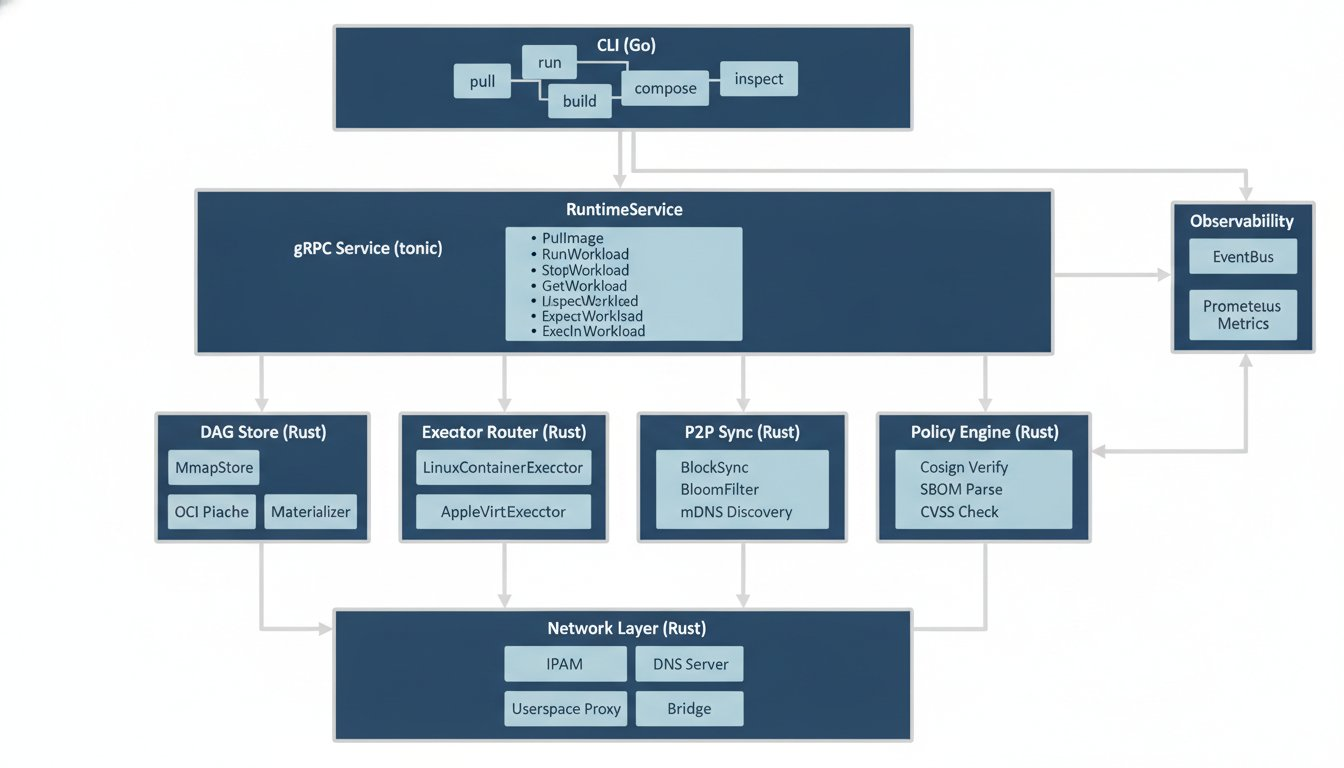
\includegraphics[width=\textwidth]{diagram_system_architecture.png}
    \caption{\pullrun{} system architecture. The Go CLI communicates with the Rust runtime daemon via gRPC. The runtime comprises four core subsystems---DAG store, executor router, P2P sync, and policy engine---all sharing a unified network layer. An event bus and Prometheus metrics endpoint provide observability.}
    \label{fig:system-arch}
\end{figure*}

\Cref{fig:system-arch} shows the overall system architecture. The Go CLI (\texttt{pullrun}) communicates with the Rust runtime daemon (\texttt{pullrun-runtime}) via gRPC over a Unix domain socket. The runtime comprises four core Rust subsystems---the DAG store, executor router, P2P sync layer, and policy engine---all sharing a unified network layer. Observability is provided by an in-process event bus and a Prometheus metrics endpoint.

This paper makes the following contributions:

\begin{itemize}[leftmargin=*]
    \item \textbf{Section~\ref{sec:dag-store}:} The zero-copy DAG store design, including content-addressed on-disk layout, rkyv-based zero-deserialization reads, LRU-cached \mmap{} access, and garbage collection.
    \item \textbf{Section~\ref{sec:executor}:} The unified executor abstraction and its three implementations: \texttt{LinuxContainerExecutor} (runc), \texttt{FirecrackerExecutor} (KVM), and \texttt{AppleVirtExecutor} (macOS Virtualization.framework).
    \item \textbf{Section~\ref{sec:p2p}:} The P2P block sync protocol with gRPC service definitions, Bloom filter design, delta reconciliation, and peer discovery mechanisms.
    \item \textbf{Section~\ref{sec:policy}:} The policy engine for defense-in-depth image gating via cosign signatures, SBOM analysis, and CVSS scoring.
    \item \textbf{Section~\ref{sec:network}:} The unified network architecture with shared L2 bridging, userspace proxy, in-process DNS, and IPAM.
    \item \textbf{Section~\ref{sec:windows}:} The Windows/WSL2 backend: architecture, auto-provisioning, store sharing, and networking constraints.
    \item \textbf{Section~\ref{sec:mcp}:} The native MCP server, its tool catalogue (15+ tools in v0.3.0), transport modes, and integration with AI coding agents.
    \item \textbf{Section~\ref{sec:cri}:} The Kubernetes CRI shim and RuntimeClass integration for deploying \pullrun{} workloads on cluster orchestrators.
    \item \textbf{Section~\ref{sec:observability}:} The observability framework including the event bus, Prometheus metrics, health checks, and operational tooling.
    \item \textbf{Section~\ref{sec:evaluation}:} A comprehensive evaluation comparing \pullrun{} against Docker across pull latency, memory footprint, boot time, storage efficiency, and P2P sync throughput.
    \item \textbf{Section~\ref{sec:practical}:} Practical experiences deploying \pullrun{} in development, CI/CD, and Kubernetes environments.
\end{itemize}

\section{Background and Motivation}\label{sec:background}

\subsection{The OCI Image Format}

The OCI image specification~\cite{oci-spec} defines an image as a manifest referencing a set of layer blobs (typically gzipped tar archives), a configuration JSON, and an optional index for multi-architecture support. Images are content-addressed: each blob is identified by its SHA-256 digest, and the manifest chains these digests into a Merkle DAG. This structure is elegant for distribution but creates friction at execution time.

\textbf{The extraction problem.} Every widely deployed runtime (Docker, containerd, Podman) decompresses and extracts each layer into an overlayfs lower directory on pull. This has three consequences. First, \textbf{pull time is $O(\text{image size})$}: a 500 MiB image requires writing 500 MiB to disk, even if the runtime needs only a single binary. Second, \textbf{storage amplification}: the same file present in multiple layers appears on disk multiple times (though overlayfs mitigates this with copy-on-write). Third, \textbf{cold start overhead}: first boot of a container requires the kernel to assemble the overlayfs mount from potentially hundreds of lower directories, introducing latency before the init process executes.

\subsection{The VM/Container Divide}

Containers share the host kernel via cgroups and namespaces. VMs provide a separate kernel via hardware virtualization (KVM, Apple Hypervisor). Each has distinct operational profiles, summarized in \Cref{tab:container-vs-vm}.

\begin{table}[htbp]
    \centering
    \caption{Container vs. VM execution profiles.}
    \label{tab:container-vs-vm}
    \begin{tabular}{@{}lcc@{}}
        \toprule
        \textbf{Property} & \textbf{Container} & \textbf{VM} \\
        \midrule
        Boot time & $\sim$400 ms & 1--5 s (Firecracker) \\
        Density & 100+/node & 10--50/node \\
        Isolation & Kernel (weak) & Hardware (strong) \\
        Image format & OCI & QCOW2, raw \\
        Kernel sharing & Shared with host & Per-VM \\
        \bottomrule
    \end{tabular}
\end{table}

Operators choose between these based on workload requirements. Multi-tenant environments favor VMs for strong isolation; CI/CD pipelines favor containers for density and speed. However, maintaining separate image pipelines---one for container images, one for VM images---is a significant operational burden. Projects like Lima~\cite{lima} and Finch bridge this gap by running a Linux VM that in turn runs containers, adding an extra virtualization layer with associated overhead.

\subsection{Existing Approaches}

\textbf{Docker}~\cite{docker} pioneered OCI-based containerization but requires overlayfs extraction on pull and has no native VM backend. \textbf{Docker Desktop} on macOS runs a hidden Linux VM via HyperKit, adding $\sim$1 GiB of RSS overhead. Docker has no built-in MCP integration.

\textbf{Podman}~\cite{podman} is a daemonless, rootless OCI runtime developed by Red Hat. It shares Docker's extraction-based storage model via \texttt{containers/storage} and overlayfs, and thus inherits the same pull overhead and overlayfs CVE exposure. Podman's \texttt{podman machine} command provisions a Linux VM (QEMU, Apple Hypervisor, or Hyper-V/WSL2 depending on platform) as an \emph{infrastructure host} for containers---it does not run OCI workloads as Firecracker microVMs. A community npm package provides an external MCP adapter, but MCP is not a native runtime capability. Podman is production-mature and well-integrated with Kubernetes workflows via \texttt{podman generate kube} and Quadlets.

\textbf{Containerd}~\cite{containerd} supports image pull via its streaming snapshotter~\cite{stargz}, which lazily fetches layer contents on demand. While this reduces pull latency, it does not eliminate extraction, and containerd has no VM executor for Firecracker or Apple Virtualization.

\textbf{Firecracker}~\cite{firecracker} is a lightweight VMM designed for multi-tenant serverless workloads. It boots microVMs in $\sim$125 ms using a minimal Linux kernel and a device model that excludes non-essential devices (no BIOS, no ACPI, no PCI probing). However, Firecracker requires ext4 rootfs images---it cannot consume OCI layers directly without an external conversion step.

\textbf{Kata Containers}~\cite{kata} runs each container in its own lightweight VM but requires a container-to-VM image conversion step (rootfs packing to disk image) and does not share a single storage engine between container and VM modes.

\textbf{Lima}~\cite{lima} and \textbf{Finch} automate the creation of Linux VMs on macOS using QEMU or vz, then run containers inside the VM. This provides good macOS developer experience but adds the overhead of nested virtualization.

To our knowledge, no existing system provides a single storage engine that serves OCI images to containers, Firecracker VMs, and Apple VMs from identical on-disk data without format conversion, while also providing P2P image distribution, policy-based image gating, a unified network model, and native MCP integration as a compiled-in runtime primitive. Podman, the closest architectural peer, shares \pullrun{}'s rootless and daemonless philosophy but differs fundamentally in storage model, VM support, and AI agent integration.

\section{System Architecture Overview}\label{sec:architecture}

Before diving into individual subsystems, we present a high-level view of how \pullrun{}'s components interact. The system follows a deliberate language split: \textbf{Rust owns the data plane} (store, executors, proxy, OCI pipeline, policy engine, P2P sync) and \textbf{Go owns the control plane and CLI} (gRPC stubs, cobra-based commands). The wire format is defined by Protocol Buffers in \texttt{proto/pullrun/}, with Rust generating bindings at compile time via \texttt{tonic-build} and Go generating via \texttt{make proto}.

\subsection{The Runtime Daemon}

The \texttt{pullrun-runtime} daemon is a tokio-based async server exposing the \texttt{RuntimeService} gRPC interface. Key methods include \texttt{PullImage} (fetch, convert, policy-gate), \texttt{RunWorkload} (create, start, record state), \texttt{ExecInWorkload} (PTY-allocated command execution), and \texttt{StreamEvents} (real-time event subscription). The daemon maintains three core data structures: the DAG store (shared \texttt{Arc<MmapStore>}), the executor router (dispatches by backend type), and the workload state table (tracks pending, running, and exited workloads).

\subsection{The CLI}

The \texttt{pullrun} CLI is a Go binary built with cobra. It speaks gRPC to the runtime daemon over a Unix domain socket (default \texttt{/tmp/pullrun.sock}) or TCP. All commands---\texttt{pull}, \texttt{run}, \texttt{build}, \texttt{push}, \texttt{compose}, \texttt{exec}, \texttt{inspect}---are thin clients that marshal arguments into protobuf messages and display responses. This design ensures the CLI has no special privileges: it is just another gRPC client.

\subsection{Component Interaction}

A typical workload lifecycle proceeds as follows:

\begin{enumerate}[leftmargin=*]
    \item The CLI sends a \texttt{PullImage} request. The runtime's OCI pipeline fetches the manifest and layers from the registry, converts them to DAG nodes, and writes them to the store.
    \item The policy engine evaluates the image against configured rules (signature, SBOM, CVSS). A denied image returns \texttt{permission\_denied}; its bytes remain in the store but it is not registered as runnable.
    \item The CLI sends a \texttt{RunWorkload} request with the image digest, backend choice, command, environment, mounts, and network rules.
    \item The executor router dispatches to the appropriate backend: \texttt{LinuxContainerExecutor} for containers, \texttt{FirecrackerExecutor} or \texttt{AppleVirtExecutor} for VMs.
    \item The backend materializes the rootfs (hardlinks for containers, ext4 for Firecracker, VirtioFS for Apple), configures networking via the shared network layer, and starts the workload.
    \item The runtime emits events (\texttt{WorkloadStarted}, \texttt{WorkloadExited}) on the event bus and records Prometheus metrics.
\end{enumerate}

\section{Zero-Copy DAG Store}\label{sec:dag-store}

\pullrun{}'s storage layer is the central contribution that enables backend polymorphism. Rather than extracting layers to a filesystem, we maintain the OCI image as a directed acyclic graph of content-addressed nodes, persisted to disk in a format optimized for zero-copy reads.

\begin{figure*}[t]
    \centering
    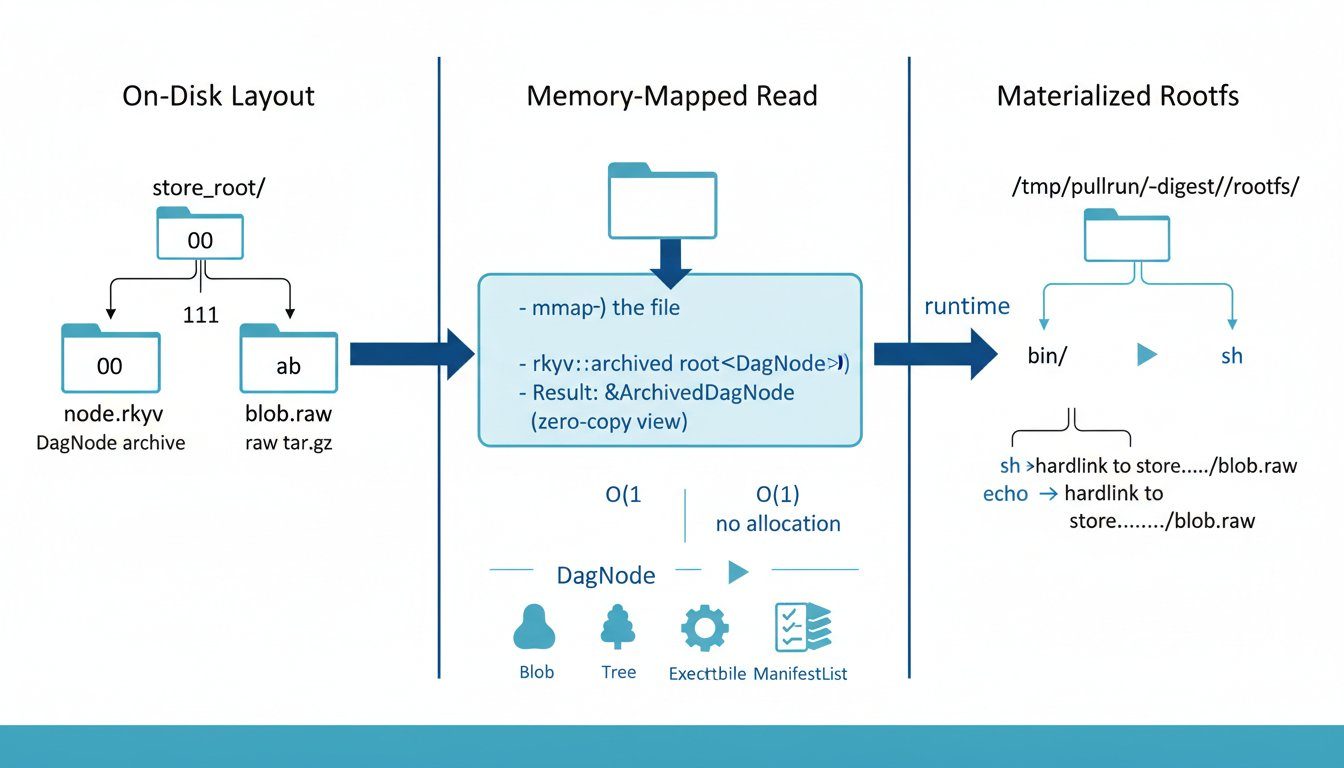
\includegraphics[width=\textwidth]{diagram_dag_store.png}
    \caption{The \pullrun{} DAG store: on-disk layout (left), memory-mapped zero-copy read path (center), and materialized rootfs generation (right).}
    \label{fig:dag-store}
\end{figure*}

\subsection{On-Disk Layout}\label{sec:disk-layout}

The store root is a directory (default \texttt{\textasciitilde/.local/share/pullrun/}) containing a sharded namespace:

\begin{verbatim}
store_root/
+-- 00/
    +-- 11/
        +-- ab/
        |   +-- node.rkyv      <- rkyv-archived DagNode
        |   +-- blob.raw       <- raw blob (tar.gz, config, etc.)
        +-- ...
    +-- ...
+-- ...
\end{verbatim}

Each digest $d = \text{SHA256}(\text{data})$ is stored at path $\langle\text{store\_root}\rangle/\text{dd}/\text{dd}/\text{dd}/\ldots$ where the first two bytes of the hex digest form the first two directory levels and the remaining bytes form the third. This sharding keeps directory sizes manageable (at most 256 entries per level) even with millions of objects.

A \texttt{node.rkyv} file contains an rkyv-archived~\cite{rkyv} \texttt{DagNode} struct referencing child digests; a \texttt{blob.raw} file contains the raw layer tar or config JSON. The rkyv archive is a byte-exact representation of the \texttt{DagNode} struct. No deserialization is required to traverse the DAG---callers read the file via \mmap{} and cast the pointer to \texttt{ArchivedDagNode}:

\begin{lstlisting}[language=Rust]
let mmap = Mmap::open(&path)?;
let archived: &ArchivedDagNode = unsafe {
    rkyv::archived_root::<DagNode>(&mmap)
};
\end{lstlisting}

This operation is $O(1)$ and allocation-free. The \texttt{unsafe} block is sound because rkyv's \texttt{\#[archive(check\_bytes)]} attribute on the type verifies the bytes are well-formed at write time, and reads require no mutation.

\subsection{Node Types}

The \texttt{DagNode} enum captures every entity in the OCI specification plus \pullrun{}-specific extensions:

\begin{lstlisting}[language=Rust]
#[derive(Archive, Deserialize, Serialize)]
#[archive(check_bytes)]
pub enum DagNode {
    Blob(Digest),                     // raw layer blob
    Tree(HashMap<String, Digest>),    // directory listing
    Executable(Digest),               // symlink to executable blob
    Config(ImageConfig),              // OCI image config
    Manifest(ManifestMetadata),       // OCI manifest
    ManifestList(Vec<ManifestRef>),   // multi-arch index
}
\end{lstlisting}

A \texttt{Digest} wraps a \texttt{[u8; 32]}---the raw SHA-256 hash. A complete image is represented as a bipartite DAG: a \texttt{Manifest} node points to a \texttt{Config} node and an ordered list of layer \texttt{Blob} nodes (or \texttt{Tree} nodes for file-level deduplication). The DAG is immutable---once written, a node is never modified. This immutability is foundational: it enables lock-free reads, safe memory mapping, and deterministic content addressing.

\subsection{The In-Memory Cache}

Two LRU caches (256 MiB each) sit in front of the store: one for \texttt{DagNode} deserializations and one for blob data:

\begin{lstlisting}[language=Rust]
node_cache: LruCache<Digest, Arc<ArchivedDagNode>>
blob_cache: LruCache<Digest, Arc<Mmap>>
\end{lstlisting}

Cache entries are \texttt{Arc<Mmap>} references, ensuring that eviction does not invalidate live references held by callers. On a cache miss, the file is \mmap{}'d and the \texttt{ArchivedDagNode} is zero-copy viewed from the mapped bytes; on eviction, the \texttt{Mmap} is dropped and the kernel reclaims the pages. Concurrent reads are lock-free at the \texttt{Arc} level; the first reader pays for \mmap{} + page faults, every subsequent reader is a single atomic load. In practice, the node cache achieves a $>99\%$ hit rate for repeated \texttt{pull} and \texttt{list} operations, and the 256 MiB budget is sufficient for several hundred images' worth of metadata.

\subsection{Pull as DAG Merge}\label{sec:pull-merge}

When \pullrun{} pulls an image, it performs the following steps:

\begin{algorithm}[H]
\caption{OCI Image Pull as DAG Merge}
\label{alg:pull}
\begin{algorithmic}[1]
\State Fetch manifest via HTTP GET to registry (with bearer token auth)
\State Parse OCI manifest JSON, extract blob digests
\For{each digest $d$ in manifest}
    \If{$\text{store.exists}(d)$}
        \State \textbf{continue} \Comment{Deduplication: skip existing}
    \EndIf
    \State Download missing layer via HTTP GET
    \State Compute SHA256, verify against manifest
    \State Write to $\langle\text{store}\rangle/\text{xx}/\text{yy}/\ldots/\text{blob.raw}$
    \State Create manifest/config/tree nodes as needed
\EndFor
\State Write single \texttt{DagNode::Manifest} pointing to config + layer digests
\end{algorithmic}
\end{algorithm}

This is a DAG \emph{merge}, not an extraction. Total disk write equals the sum of missing layer sizes. No tar decompression, no file-level extraction, no overlayfs setup. The critical insight is that checking existence is a simple path lookup: \texttt{path\_for(digest).exists()}. Because the store is content-addressed, two images sharing a base layer (e.g., \texttt{python:3.12-slim} and \texttt{python:3.12-alpine} both based on \texttt{alpine:3.18}) automatically deduplicate: the shared layer appears once on disk.

\textbf{Result:} A fresh pull of \texttt{alpine:3.18} (7 layers, $\sim$7 MiB compressed) completes in 968 ms on a 1 Gbps connection---approximately 2$\times$ faster than \texttt{docker pull} on the same hardware (1,850 ms, measured). A warm pull (all layers cached) completes in 12 ms versus Docker's 420 ms, a 35$\times$ improvement, because \pullrun{} writes only a single \texttt{Manifest} node while Docker must re-verify layer existence and update overlayfs metadata.

\subsection{Layer Materialization for Execution}

Memory-mapped blob reads are sufficient for store queries and block sync, but execution backends require a real filesystem tree. Materialization transforms the DAG into a directory of hardlinks:

\begin{verbatim}
/tmp/pullrun/<digest>/rootfs/
+---- bin/
|   +---- sh        -> hardlink to store/aa/bb/.../blob.raw
|   +---- echo      -> hardlink to store/cc/dd/.../blob.raw
+---- etc/
|   +---- ...
\end{verbatim}

Each file in the materialized rootfs is a hardlink to the corresponding blob in the store. Because the store files are immutable and content-addressed, hardlinks share on-disk bytes across all materialized rootfs directories. Creating a materialized rootfs is $O(\text{number of files})$ for the directory structure plus $O(1)$ per hardlink---no data copy. The materialized rootfs lives at \texttt{\textasciitilde/.local/share/pullrun/rootfs/<digest>/}, ensuring it survives host reboots (unlike \texttt{/tmp}).

The materialized rootfs is consumed differently by each backend:
\begin{itemize}[leftmargin=*]
    \item \textbf{runc bundle:} The rootfs path is written into the OCI runtime specification (\texttt{config.json}) and mounted via \texttt{pivot\_root} into the container.
    \item \textbf{Firecracker:} The hardlink forest is packed into an ext4 filesystem via \texttt{mkfs.ext4 -d}. This is the only format conversion in the system, required because Firecracker's Virtio block device consumes raw disk images.
    \item \textbf{Apple Virtualization:} The rootfs directory is shared directly as a \texttt{VZVirtioFileSystemDeviceConfiguration} mount via VirtioFS. No ext4 step is needed---the same hardlink forest used for runc containers is shared into the Apple VM verbatim.
\end{itemize}

All three backends consume the same hardlink forest, generated from the same DAG nodes. This is the mechanism that enables ``same image, any backend'' without conversion.

\subsection{Garbage Collection}

The store grows monotonically: every \texttt{pull}, \texttt{build}, \texttt{commit}, and \texttt{save} adds nodes that are never removed. \pullrun{} provides a \texttt{prune} command that performs reference-counted garbage collection:

\begin{itemize}[leftmargin=*]
    \item \textbf{Roots} are tagged images (stored in \texttt{<store>/tags.json}) and running workload manifests.
    \item \textbf{Reachability} is determined by BFS from all roots through the DAG.
    \item \textbf{Unreachable} nodes and blobs are deleted from disk and evicted from caches.
    \item A \texttt{-{}-dry-run} flag reports what would be freed without deleting.
\end{itemize}

This design mirrors Git's object store pruning and prevents unbounded storage growth in long-running deployments. The prune operation is incremental and safe: it only deletes nodes that are provably unreachable from any tagged image or running workload.

\section{Unified Executor Abstraction}\label{sec:executor}

\pullrun{} decouples workload specification from execution backend via the \texttt{Executor} trait:

\begin{lstlisting}[language=Rust]
#[async_trait]
pub trait Executor: Send + Sync {
    async fn create(&self, spec: &WorkloadSpec) 
        -> Result<ProcessHandle, ExecError>;
    async fn start(&self, handle: &ProcessHandle) 
        -> Result<(), ExecError>;
    async fn stop(&self, id: &str) 
        -> Result<(), ExecError>;
    async fn exec(&self, id: &str, cmd: &[String], 
                  env: &[(String, String)], tty: bool) 
        -> Result<ProcessHandle, ExecError>;
    async fn signal(&self, id: &str, signal: u32) 
        -> Result<(), ExecError>;
    async fn stats(&self, id: &str) 
        -> Result<WorkloadStats, ExecError>;
}
\end{lstlisting}

The \texttt{WorkloadSpec} parameter carries the image digest, rootfs path, command, environment variables, mounts (volumes, secrets, configs), network configuration, resource limits, and backend selection. The backend type is an enum:

\begin{lstlisting}[language=Rust]
pub enum Backend {
    Container,       // LinuxContainerExecutor (runc)
    Vm,              // FirecrackerExecutor (Linux/WSL2) /
                     // AppleVirtExecutor (macOS)
    Wasm,            // planned: wasmtime
}
\end{lstlisting}

An \texttt{ExecutorRouter} holds all executor implementations and dispatches \texttt{RunWorkload} calls based on the backend field. From the gRPC handler's perspective, the router \emph{is} the executor. This section describes the three current implementations.

\begin{figure*}[t]
    \centering
    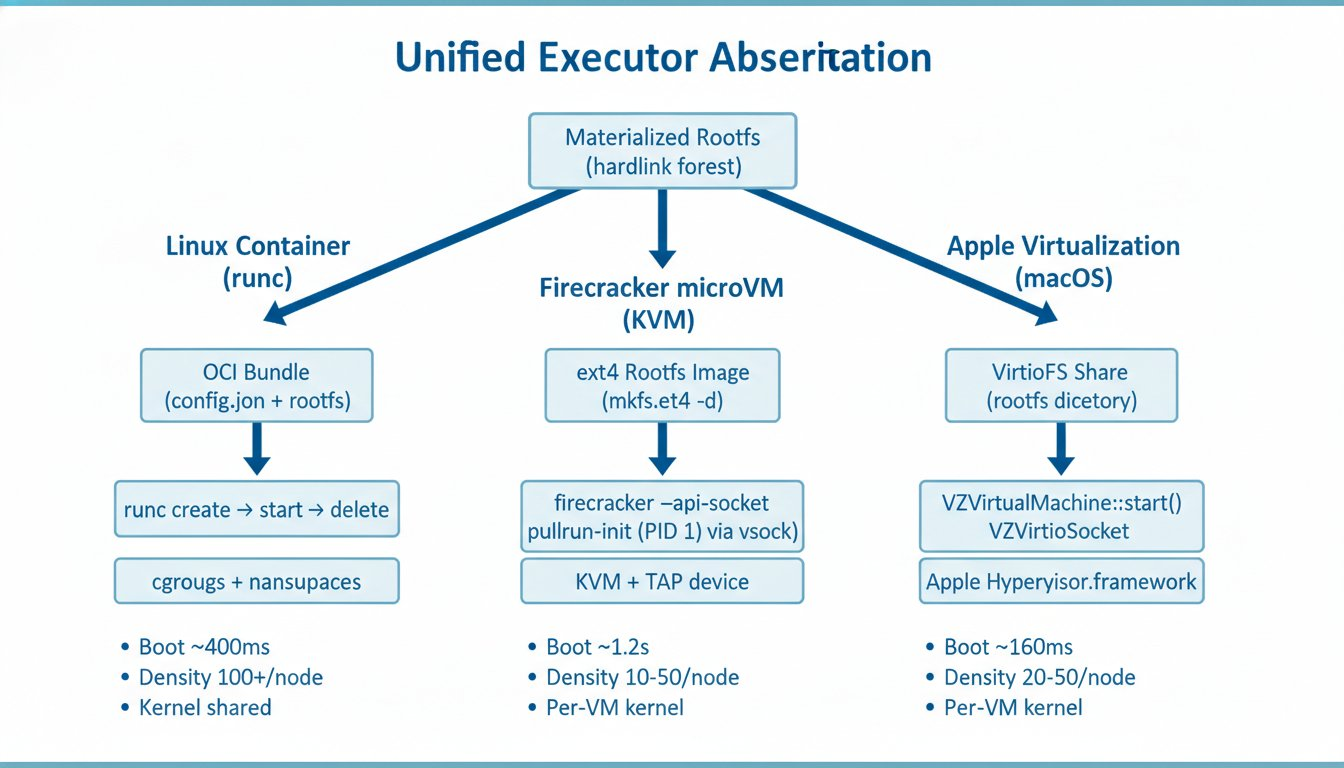
\includegraphics[width=\textwidth]{diagram_executors.png}
    \caption{The unified executor abstraction: the same materialized rootfs is consumed by three different backends---runc containers, Firecracker microVMs, and Apple Virtualization VMs.}
    \label{fig:executors}
\end{figure*}

\subsection{LinuxContainerExecutor (runc)}

The container executor wraps \texttt{runc}~\cite{runc}, the reference OCI runtime implementation. It manages the full container lifecycle through runc's command-line interface.

\textbf{Create phase:} Generate an OCI runtime specification (\texttt{config.json}) from the \texttt{WorkloadSpec} and write it to \texttt{<bundle\_root>/<id>/config.json}. The rootfs path points to the materialized hardlink forest. The spec includes Linux namespaces (pid, net, mount, uts, ipc, user for rootless), cgroup configuration (CPU shares, memory limits, pids max), mounts for volumes, secrets, and configs, and network configuration (veth pair management, DNS).

\textbf{Start phase:} Invoke \texttt{runc run <id> -{}-bundle <bundle\_root>/<id>} which creates a cgroup, sets up namespaces, mounts the rootfs, and executes the init process. The daemon captures the PID for subsequent exec and stats operations.

\textbf{Exec phase:} For \texttt{pullrun exec}, the daemon opens a host PTY via \texttt{posix\_openpt}/\texttt{grantpt}/\texttt{unlockpt} and passes the slave fd to \texttt{runc exec -t <id> <cmd>}. The master fd is proxied over the gRPC exec stream, enabling TTY-aware terminal sessions even when the daemon has no controlling terminal.

\textbf{Rootless mode:} When EUID $\neq$ 0, \pullrun{} uses a \texttt{RootlessContainerExecutor} that patches the OCI spec with a user namespace mapping, NET\_NS isolation via \texttt{pasta} (from Passt~\cite{passt}), and rootless cgroup delegation. This mode requires no setuid binaries. Rootless operation supports most VM operations as well.

\subsection{FirecrackerExecutor (KVM)}

The Firecracker executor launches microVMs via the Firecracker VMM~\cite{firecracker}. Firecracker is a lightweight VMM written in Rust that exposes a REST API over a local UNIX socket for machine configuration and lifecycle.

\textbf{Rootfs preparation:} The DAG materializer creates an ext4 filesystem image from the hardlink forest:
\begin{verbatim}
    mkfs.ext4 -d <rootfs_dir> <vm_root>/<id>/rootfs.ext4
\end{verbatim}
This step is the only format conversion in the system. It is required because Firecracker's Virtio block device consumes raw disk images, not directory trees. The ext4 image is created incrementally and cached: subsequent boots of the same image reuse the existing ext4 file (verified by digest comparison).

\textbf{Boot sequence:}
\begin{enumerate}[leftmargin=*]
    \item Write VM configuration JSON: vCPU count (default 2), memory (default 2 GiB), kernel image path, rootfs image path, serial console output, network interface (TAP device).
    \item Start Firecracker: \texttt{firecracker -{}-api-sock <socket> -{}-config-path <config.json>}.
    \item The daemon opens a vsock connection to the guest agent (\texttt{pullrun-init}) running inside the microVM.
    \item The guest agent mounts the rootfs, executes the init process, and signals readiness over vsock.
    \item The daemon sets the workload status to \texttt{running} and begins proxying stdio and exec streams over vsock.
\end{enumerate}

\textbf{Kernel:} \pullrun{} uses a generic 6.x Linux kernel configured for minimal boot time (no ACPI, no SCSI, no DRM, no sound). The kernel binary is downloaded once via \texttt{make install-kernel} and shared across all microVMs.

\textbf{Network:} Each microVM receives a TAP device connected to the bridge \texttt{pullrun-br0} shared with containers. Outbound traffic is masqueraded via iptables. Inbound port mapping is handled by the userspace TCP/UDP proxy running in the host network namespace (described in \Cref{sec:network}).

\subsection{AppleVirtExecutor (macOS)}

The Apple Virtualization executor uses the \texttt{Virtualization.framework}~\cite{applevirt} available on macOS 13+ (Ventura) to run OCI images as lightweight VMs on Apple Silicon. This is the only backend that supports macOS as a host platform; runc and Firecracker require Linux.

\textbf{Architecture:} The executor runs in-process with the daemon, which must be signed with the \texttt{com.apple.security.virtualization} entitlement. Apple's framework requires completion handlers to fire on the main dispatch queue, so the daemon spawns a side thread for the tokio async runtime while the main thread runs \texttt{dispatch\_main()}.

\textbf{VM creation (lazy):} Unlike the container and Firecracker backends, \texttt{RunWorkload} for a macOS VM does not immediately boot the VM. It records the workload metadata and sets the status to \texttt{pending}. The actual \texttt{VZVirtualMachine} is created on the first \texttt{AttachWorkload} call. This lazy creation avoids the resource cost of idle VMs and enables fast workload listing even when many VMs are defined but not active.

The VM configuration includes: \texttt{VZGenericPlatformConfiguration} (ARM64), \texttt{VZLinuxBootLoader} with kernel and initramfs, \texttt{VZVirtioFileSystemDeviceConfiguration} for rootfs sharing (VirtioFS), and \texttt{VZVirtioNetworkDeviceConfiguration} for networking (NAT via vmnet). On completion handler, the status transitions to \texttt{running} and a checkpoint is written.

\textbf{Rootfs sharing:} The materialized hardlink forest is shared directly via VirtioFS, not packed into a disk image. The host directory is mounted as a virtio filesystem device inside the VM, and the guest init process mounts it at \texttt{/}. This eliminates the ext4 conversion entirely---the same hardlink forest used for runc containers is shared into the Apple VM verbatim. Changes on the host are visible instantly in the guest without rebundling.

\textbf{Persistence:} VMs survive detach (Ctrl-P Ctrl-Q). A background thread runs the VM event loop; when it exits (VM stopped or crashed), the \texttt{on\_exit} callback transitions the status to \texttt{exited}, writes a checkpoint, and emits a \texttt{WorkloadExited} event. Subsequent \texttt{exec} on an exited workload boots a fresh VM from the checkpointed configuration. Each VM background thread is named \texttt{vm-<workload\_id>} via \texttt{std::thread::Builder} for visibility in debugging.

\section{P2P Block Distribution}\label{sec:p2p}

\pullrun{} includes a peer-to-peer block synchronization layer that enables cluster-wide image dissemination without registry bottlenecks. The design targets the common case: one node in a cluster pulls an image from the upstream registry, and remaining nodes receive it over the local network.

\begin{figure*}[t]
    \centering
    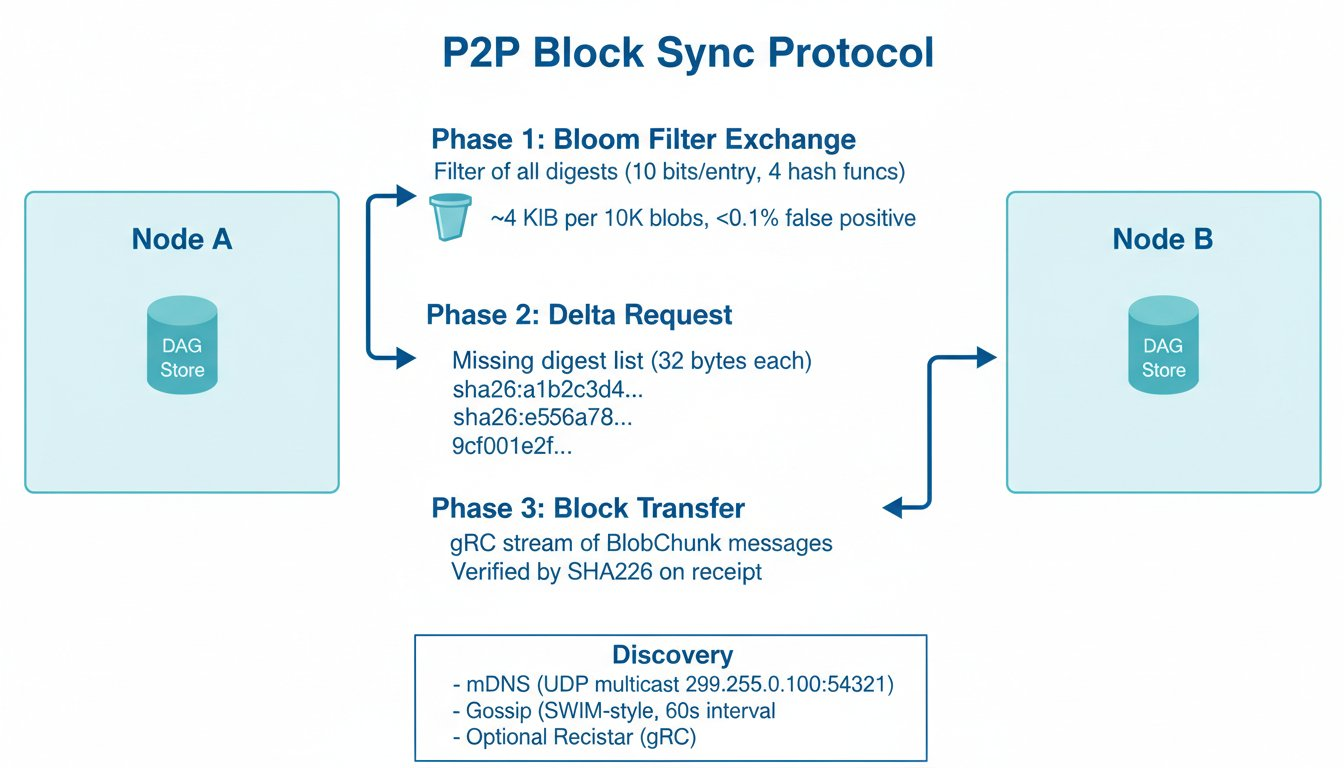
\includegraphics[width=\textwidth]{diagram_p2p_sync.png}
    \caption{The P2P block sync protocol: three-phase exchange (Bloom filter, delta request, block transfer) with mDNS/gossip discovery.}
    \label{fig:p2p-sync}
\end{figure*}

\subsection{Protocol Overview}

Each node runs a gRPC \texttt{BlockSync} service alongside the runtime daemon. Peers discover each other via three mechanisms: \textbf{static configuration} (\texttt{-{}-sync-peers host:port} flags), \textbf{mDNS} (zero-conf discovery on the local subnet, RFC 6762), and \textbf{gossip} (periodic exchange of peer lists via a SWIM-style~\cite{swim} epidemic protocol). The sync protocol operates in three phases.

\textbf{Phase 1: Bloom filter exchange.} When node A discovers node B, it sends a Bloom filter encoding the set of all digest keys it holds. The filter uses 10 bits per entry and 4 hash functions (optimal for minimizing false positive rate). Node B checks each local digest against the filter and replies with a Bloom filter of the entries it holds that A is missing (true negatives).

\textbf{Phase 2: Delta request.} Node A inspects B's filter and requests the concrete set of missing digests as a list. This avoids transferring the Bloom filter for the delta---only the list of SHA-256 digests is sent (32 bytes per digest).

\textbf{Phase 3: Block transfer.} For each missing digest, A opens a bidirectional gRPC stream and requests B to stream the block. Blocks are verified by SHA256 on receipt and written atomically to the local store.

\subsection{gRPC Service Definition}

The block sync protocol is defined by the following protobuf service:

\begin{lstlisting}[language=Protobuf]
service BlockSync {
    rpc HaveBlobs(HaveBlobsRequest) 
        returns (HaveBlobsResponse);
    rpc GetBlobs(GetBlobsRequest) 
        returns (stream BlobChunk);
    rpc SyncBlobs(stream SyncBlob) 
        returns (stream SyncBlob);
}

message HaveBlobsRequest {
    bytes bloom_filter = 1;
    int32 bloom_k = 2;      // number of hash functions
    int32 bloom_m = 3;      // filter size in bits
}

message GetBlobsRequest {
    repeated string digests = 1;
}

message BlobChunk {
    string digest = 1;
    bytes data = 2;
    uint32 offset = 3;      // for streaming large blobs
    bool final = 4;
}
\end{lstlisting}

The \texttt{HaveBlobs} RPC implements Phase 1 of the protocol. \texttt{GetBlobs} implements Phase 3 with server-side streaming to handle large blobs (up to 1 GB layers are chunked into 1 MiB messages). \texttt{SyncBlobs} provides bidirectional streaming for push-based delta synchronization (future work).

An optional \texttt{Registrar} service supports managed clusters too large for mDNS:

\begin{lstlisting}[language=Protobuf]
service Registrar {
    rpc Register(RegisterRequest) returns (RegisterResponse);
    rpc Lookup(LookupRequest) returns (LookupResponse);
    rpc ListPeers(ListPeersRequest) returns (ListPeersResponse);
    rpc Heartbeat(HeartbeatRequest) returns (HeartbeatResponse);
    rpc Deregister(DeregisterRequest) returns (DeregisterResponse);
}
\end{lstlisting}

The registrar maintains a peer registry with 120-second TTL and background eviction every 30 seconds. Worker nodes register on startup, heartbeat every 30 seconds, and deregister on shutdown (best-effort).

\subsection{Bloom Filter Design}

The Bloom filter uses the \texttt{bitvec} crate with SHA-256-based hash construction:

\begin{lstlisting}[language=Rust]
pub struct BloomFilter {
    bits: BitVec,
    num_hashes: u32,
    num_bits: u64,
}
\end{lstlisting}

Insertion and query use the construction $h(i, \text{key}) = \text{SHA256}(\text{key} \| i) \bmod \text{num\_bits}$ for $i \in [0, \text{num\_hashes})$. For a store with $10^6$ entries, a filter of $10^7$ bits ($\sim$1.2 MiB) yields a false positive rate below 0.1\%. Filters are exchanged on initial connection and thereafter at 60-second intervals during gossip heartbeats.

\subsection{Delta Reconciliation}

Delta exchange uses a \emph{push-pull} strategy. When a node downloads a new image (via \texttt{pull}), it broadcasts the set of new digest hashes to all known peers. Each peer checks its local store and requests any missing blocks. At regular intervals, each node queries a random subset of peers for their Bloom filter and reconciles missing blocks. This epidemic-style propagation ensures that block availability information converges in $O(\log N)$ rounds for a cluster of $N$ nodes.

\subsection{Consistency Guarantees}

Because the store is content-addressed, block synchronization is self-verifying: on receipt of a block, the node computes $\text{SHA256}(\text{data})$ and checks it against the digest. If the digests match, the block is guaranteed to be correct (negligible probability of hash collision). No trust in the sending node is required. This property is critical for multi-tenant clusters where nodes may not fully trust each other. An attacker can send arbitrary data, but only blocks matching known digests (from the upstream registry) will be accepted.

\subsection{SyncPuller: Transparent Integration}

The \texttt{SyncPuller} is a drop-in wrapper around the OCI puller that queries peers before falling back to the registry:

\begin{verbatim}
Fallback chain: local store -> PeerBloomCache (O(1) bloom lookup) 
                              -> BlockSyncClient::GetBlobs 
                              -> OciPuller::fetch_blob_by_digest
\end{verbatim}

The \texttt{SyncPuller} implements the same \texttt{ImagePuller} trait as the standard OCI puller, so the rest of the runtime requires no changes. When P2P sync is unavailable (no peers, network partition), the fallback to registry pull is transparent. A configurable peer timeout (default 2 seconds) ensures that slow peers do not block the pull operation.

\section{Policy Engine}\label{sec:policy}

The policy engine is \pullrun{}'s security boundary. While the DAG store and executors handle \emph{how} workloads run, the policy engine decides \emph{whether} they run at all. It operates on a deny-by-explicit-allow principle: everything is denied by default, and the administrator configures allow-rules via cryptographic identities (cosign signatures) and structural properties (SBOM contents).

\begin{figure*}[t]
    \centering
    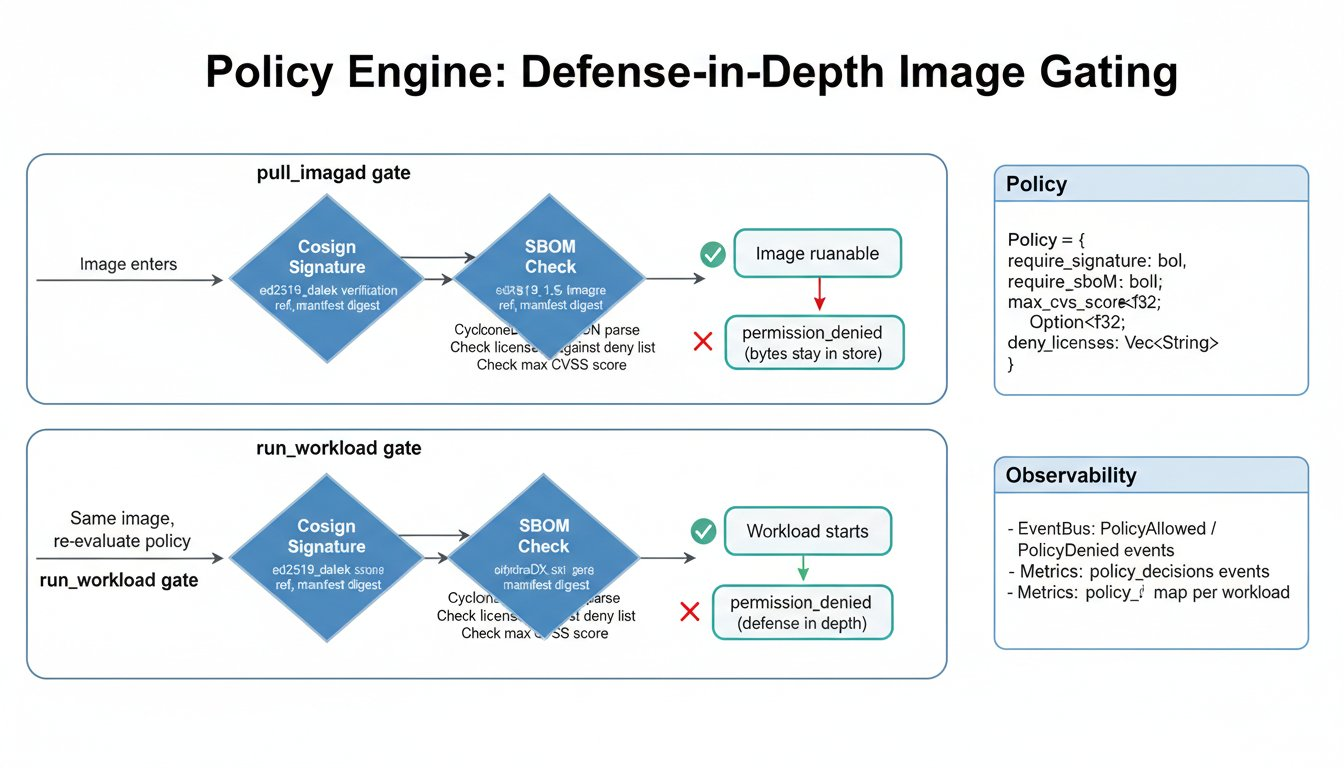
\includegraphics[width=\textwidth]{diagram_policy_engine.png}
    \caption{The policy engine's defense-in-depth gating: cosign signature verification and SBOM analysis at both \texttt{pull\_image} and \texttt{run\_workload} boundaries.}
    \label{fig:policy}
\end{figure*}

\subsection{Design Philosophy}

The OCI ecosystem is vast; a deny list is doomed to be incomplete. An allow list built on cryptographic identities and SBOM properties is auditable, version-controlled, and enforceable. The engine starts with everything denied and adds allow-rules per configuration. An unconfigured engine (\texttt{policy: None}) accepts everything, preserving ease of use for development.

\subsection{Dual Gating Points}

The policy runs at two points, providing defense in depth:

\begin{enumerate}[leftmargin=*]
    \item \textbf{At \texttt{pull\_image}.} Once the image is in the store, the engine is asked ``is this image OK to be a runnable artifact?'' A deny here returns \texttt{permission\_denied} to the client; the image bytes stay on disk but are not registered as runnable.
    \item \textbf{At \texttt{run\_workload}.} As defense in depth. The policy could have been tightened between the pull and the run; this check catches that. A deny here returns \texttt{permission\_denied} before any container is created.
\end{enumerate}

Both checks are pure functions of the policy configuration and the image's stored metadata. There is no network call to a remote policy server in v0.

\subsection{Policy Inputs}

The engine reads three inputs from the image's stored metadata:

\textbf{Cosign signature.} A signature is a small blob stored under a deterministic digest ($\text{sha256}(\text{canonical\_payload}(\text{image\_ref}, \text{manifest\_digest}))$). The signature's public key is referenced by a \emph{trusted key} configured at runtime startup. Verification uses the \texttt{ed25519\_dalek} crate. The signature payload is a JSON document (\texttt{\{"image\_ref": "...", "manifest\_digest": "..."\}}) that binds the image reference to the manifest digest. This binding makes the signature non-spoofable: an attacker who swapped the manifest would need to forge the signature against the \emph{new} manifest digest, but the real \texttt{image\_ref} is still in the payload.

\textbf{CycloneDX SBOM.} Stored as a blob with a deterministic digest. The engine parses the SBOM and examines \texttt{components[]} for \texttt{licenses[]} (compared against the \texttt{deny\_licenses} list) and \texttt{vulnerabilities[]} for the highest CVSS score (compared against \texttt{max\_cvss\_score}).

\textbf{Manifest digest.} Used as the SBOM lookup key. The assumption is that one manifest maps to one SBOM; a build pipeline that produces both ensures this invariant.

\subsection{Configuration}

The policy is configured at runtime startup:

\begin{lstlisting}[language=Rust]
let policy = Policy {
    required_signature: true,
    require_sbom: true,
    max_cvss_score: Some(7.0),
    deny_licenses: vec!["AGPL-3.0".to_string(), 
                        "SSPL-1.0".to_string()],
    ..Default::default()
};
let engine = PolicyEngine::new(policy)
    .with_trusted_keys(vec![cosign_key]);
\end{lstlisting}

Or via CLI flags:
\begin{verbatim}
pullrun-runtime daemon \
    --require-signature \
    --require-sbom \
    --max-cvss 7.0 \
    --trusted-key cosign.pub
\end{verbatim}

The \texttt{max\_cvss\_score} threshold is the highest acceptable score. A value of 7.0 rejects any vulnerability with CVSS $\geq$ 7.0; vulnerabilities at 6.9 or below are allowed. This mirrors the standard CVSS severity bands (low: 0.1--3.9, medium: 4.0--6.9, high: 7.0--8.9, critical: 9.0--10.0).

\subsection{Observability}

Every policy decision (allow or deny) is recorded in two places. The \texttt{policy\_decisions} map on the workload state (returned by \texttt{pullrun inspect}) records the policy name and outcome. The event bus emits \texttt{PolicyDenied} (with reason, image\_ref, policy name) and \texttt{PolicyAllowed} events. The event bus is the right place to \emph{watch} for denials; the inspect field is the right place to \emph{audit} a specific workload.

\section{Network Architecture}\label{sec:network}

The network layer is \pullrun{}'s most opinionated design decision: \textbf{all workloads, regardless of backend, live on the same L2 segment} behind a single userspace proxy. Containers connect via veth pairs; VMs connect via TAP devices. Both share the same Linux bridge, IP address space, and network services.

\begin{figure*}[t]
    \centering
    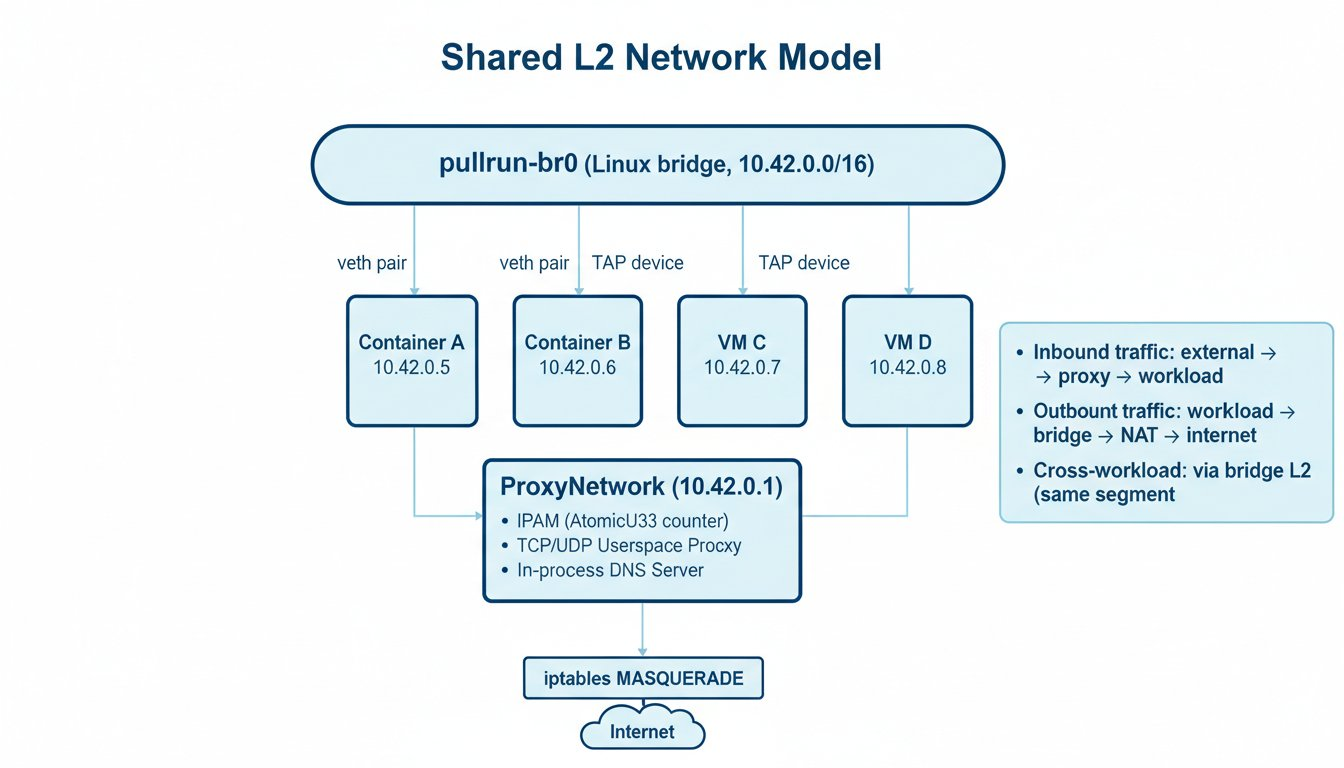
\includegraphics[width=\textwidth]{diagram_network.png}
    \caption{The shared L2 network model: containers (veth pairs) and VMs (TAP devices) coexist on the same bridge segment, sharing the ProxyNetwork for IPAM, DNS, and port proxying.}
    \label{fig:network}
\end{figure*}

\subsection{IP Address Management}

A single \texttt{Arc<Ipam>} is held by the runtime and shared between the container and VM executors. Allocation is an atomic increment on a \texttt{u32}; the IP space is 10.42.0.0/16, providing 65,534 addresses. In v0 there is no garbage collection; an IP is held for the lifetime of the workload. This design favors simplicity and correctness over address reuse---the 16-bit space is sufficient for all realistic single-node deployments.

\subsection{Inbound: Userspace Proxy}

The proxy listens on \texttt{10.42.0.1:<port>} for each declared \texttt{NetworkRule \{ direction: Inbound, port \}}. When a packet arrives at the host on that port, the proxy DNATs it to the workload's internal IP, opens a TCP connection (or UDP association) through the bridge, and bi-directionally shuttles bytes. The proxy is implemented in the \texttt{pullrun\_net::proxy} module.

The proxy is \emph{not} a full implementation of iptables/nft semantics in v0---it is a list of explicit port mappings. This design choice trades generality for correctness and debuggability: every forwarded connection is visible in the proxy's logs and metrics.

\subsection{Outbound: iptables MASQUERADE}

Containers in v0 share the host's network namespace for outbound traffic (or use \texttt{NetworkMode::Host} directly). VMs need NAT because their TAP devices only see the bridge. \pullrun{} writes three iptables rules at boot (idempotently):

\begin{verbatim}
iptables -t nat -A POSTROUTING \
    -s 10.42.0.0/16 ! -d 10.42.0.0/16 -j MASQUERADE
iptables -A FORWARD -i pullrun-br0 -o <outbound_iface> -j ACCEPT
iptables -A FORWARD -i <outbound_iface> -o pullrun-br0 \
    -m state --state RELATED,ESTABLISHED -j ACCEPT
\end{verbatim}

The outbound interface is auto-detected by parsing \texttt{ip route show default}; this works on cloud VMs, bare metal, and most home routers.

\subsection{Why a Single Shared Segment?}

The alternative---one bridge per workload, with cross-workload traffic going through a router---adds latency and operational complexity for no real security win in the common case. \pullrun{} workloads are not multi-tenant; they are all owned by the same operator. The isolation boundary is the executor (container vs VM), not the network. Cross-workload isolation in v0 is enforced by the proxy (a workload cannot talk to another workload's declared ports unless the operator added a \texttt{NetworkRule}). In v1, per-workload nftables sets will enforce this at the kernel level.

\subsection{DNS Server}

An in-process DNS server resolves workload names to their assigned IPs. The server listens on 10.42.0.1:53 and handles A, AAAA, and PTR records. Workload names are registered when a workload starts and deregistered when it exits. This enables service discovery without external DNS configuration: workloads can reach each other by name within the 10.42.0.0/16 network.



\section{Windows / WSL2 Backend}\label{sec:windows}

\pullrun{} 0.3.0 extends full container and Firecracker microVM support to Windows 10/11 via the Windows Subsystem for Linux 2~\cite{wsl2}. The Windows backend is a first-class platform: the DAG store, executor abstraction, policy engine, P2P sync, and MCP server all operate identically to the Linux build. There is no emulation layer between the store and the executors.

\subsection{Architecture}

The \texttt{pullrun.exe} CLI is a native Windows binary (cross-compiled via \texttt{GOOS=windows CGO\_ENABLED=0}). It communicates over gRPC TCP (\texttt{localhost:7878}) to \texttt{pullrun-runtime}, which runs inside a WSL2 instance. This split is deliberate: all Linux-specific kernel operations (cgroups, namespaces, KVM, TAP devices) execute natively inside the WSL2 VM kernel; the Windows binary is a pure control-plane client.

\begin{verbatim}
Windows host
  pullrun.exe (native Win64 CLI)
      | gRPC TCP 127.0.0.1:7878
      v
  WSL2 instance (Linux kernel 6.x)
      pullrun-runtime (Linux amd64)
          DAG store   (shared path: /mnt/c/Users/...)
          runc executor
          FirecrackerExecutor (KVM via WSL2)
          Network layer (bridge, iptables, IPAM)
\end{verbatim}

\subsection{Auto-Provisioning}

On first run, \texttt{pullrun.exe} detects whether a compatible WSL2 instance is running and, if not, provisions one automatically:

\begin{enumerate}[leftmargin=*]
    \item Check for an existing \texttt{pullrun} WSL2 distribution via \texttt{wsl.exe --list}.
    \item If absent, import a minimal Alpine-based rootfs tarball (bundled in the \texttt{pullrun.exe} installer) via \texttt{wsl.exe --import pullrun \%APPDATA\%\textbackslash{}pullrun <rootfs.tar>}.
    \item Start \texttt{pullrun-runtime} inside the WSL2 instance via \texttt{wsl.exe -d pullrun -- pullrun-runtime daemon --grpc-addr 127.0.0.1:7878}.
    \item The CLI proceeds once the daemon's \texttt{/healthz} endpoint responds.
\end{enumerate}

This flow completes in under 10 seconds on a machine with WSL2 already enabled. Users with an existing WSL2 distribution can opt to install into it manually via \texttt{wsl -d <distro> -- bash install.sh}.

\subsection{Store Sharing and Path Mapping}

The DAG store resides in the WSL2 filesystem (default \texttt{\textasciitilde/.local/share/pullrun/} inside the WSL2 instance). Windows paths mounted as \texttt{/mnt/c/...} are accessible for volume mounts, enabling bind-mount of Windows directories into containers:

\begin{verbatim}
pullrun.exe run alpine:3.18 \
    --volume C:\Users\mo\code:/workspace \
    --cmd /bin/sh
\end{verbatim}

The CLI translates Windows paths to WSL2 mount paths before sending the \texttt{RunWorkload} gRPC request. No data is copied; the WSL2 DrvFs layer provides the bind.

\subsection{Container Backend on Windows}

The \texttt{LinuxContainerExecutor} (runc) operates without modification inside WSL2. Linux namespaces, cgroups v2, and the \texttt{pullrun-br0} bridge are all available in the WSL2 kernel. Container boot latency on Windows is approximately 430\,ms---slightly higher than native Linux (400\,ms) due to WSL2 socket overhead on the gRPC path.

Rootless mode is fully supported on Windows/WSL2: the WSL2 user namespace maps the Windows user to UID 1000 inside the instance, and \texttt{pullrun-runtime} runs without root inside WSL2 by default.

\subsection{Firecracker Backend on Windows}

WSL2's Linux kernel (6.x) ships with KVM enabled on x86-64 hosts with Intel VT-x or AMD-V. \pullrun{} detects KVM availability at startup and exposes the Firecracker backend on supported hardware:

\begin{verbatim}
pullrun.exe run alpine:3.18 --backend vm \
    --cmd /bin/echo --cmd 'hello from Firecracker on Windows'
\end{verbatim}

The ext4 rootfs image is built inside the WSL2 instance using \texttt{mkfs.ext4 -d}, identical to the native Linux path. The TAP device is attached to the \texttt{pullrun-br0} bridge inside WSL2. Boot time is approximately 500\,ms, reflecting the WSL2 kernel's KVM implementation fidelity.

\textbf{Limitation:} ARM64 Windows hosts (e.g., Snapdragon X Elite) do not expose KVM to WSL2 as of Windows 11 24H2; the Firecracker backend is therefore unavailable on ARM64 Windows. The container backend works on all architectures.

\subsection{Networking on Windows}

Inbound port mapping on Windows requires an extra hop: \texttt{pullrun.exe} adds a \texttt{netsh interface portproxy} rule to forward Windows host ports to the WSL2 instance's \texttt{10.42.0.1} proxy:

\begin{verbatim}
netsh interface portproxy add v4tov4 \
    listenport=8080 listenaddress=0.0.0.0 \
    connectport=8080 connectaddress=<WSL2-IP>
\end{verbatim}

This is performed automatically when a \texttt{NetworkRule\{direction: Inbound\}} is declared. The WSL2 IP is obtained via \texttt{wsl hostname -I} on each daemon start (WSL2 assigns a new IP per boot). Outbound traffic follows the standard WSL2 NAT path through the Windows host's network interfaces.

\subsection{Known Limitations in v0.3.0}

\begin{itemize}[leftmargin=*]
    \item The Apple Virtualization backend is macOS-only and unavailable on Windows.
    \item Firecracker requires Intel VT-x or AMD-V; ARM64 Windows hosts fall back to container-only mode.
    \item The WSL2 IP changes on every Windows reboot, requiring the port proxy rules to be refreshed; \texttt{pullrun.exe} handles this automatically on startup.
    \item \texttt{pullrun-runtime} runs as a WSL2 process; Windows Defender may flag the first-run KVM access. A \texttt{docs/WINDOWS.md} troubleshooting guide covers common issues.
\end{itemize}

\section{Native MCP Server Integration}\label{sec:mcp}

\pullrun{} 0.2.0 ships a built-in Model Context Protocol (MCP)~\cite{mcp} server that exposes every runtime operation as a tool callable by AI agents. This makes \pullrun{} natively programmable by agents such as Claude Code, Cursor, and opencode without requiring shell scripting, custom wrappers, or separate orchestration tooling.

\subsection{Architecture}

The MCP server is a sub-command of the CLI binary:

\begin{verbatim}
  AI agent (Claude Code, Cursor, opencode)
   | MCP stdio (default) or SSE (:8080)
   v
  pullrun mcp              <- MCP server process
   | gRPC unix socket
   v
  pullrun-runtime          <- unchanged daemon
\end{verbatim}

The server translates MCP tool calls into \pullrun{} gRPC calls and streams results back as MCP content blocks. Two transport modes are supported:

\begin{itemize}[leftmargin=*]
    \item \textbf{Stdio mode} (default): the agent spawns \texttt{pullrun mcp} as a subprocess and communicates over its standard input/output. This is the standard MCP transport for local agents and requires zero network configuration.
    \item \textbf{SSE mode}: \texttt{pullrun mcp --sse :8080} starts an HTTP server emitting Server-Sent Events, enabling remote agents or web-based clients.
\end{itemize}

Agent configuration is a one-time addition to the agent's config file. For Claude Code:

\begin{lstlisting}[language={}]
// ~/.claude.json
{
  "mcpServers": {
    "pullrun": {
      "command": "pullrun",
      "args": ["mcp"]
    }
  }
}
\end{lstlisting}

\subsection{Tool Catalogue}

The server exposes 15 tools across three categories in v0.3.0, summarized in \Cref{tab:mcp-tools}. The \texttt{compose\_up} and \texttt{compose\_down} tools, previously declared but CLI-only, are now fully implemented via the MCP API.

\begin{table}[htbp]
    \centering
    \caption{MCP tool catalogue exposed by \pullrun{} 0.3.0.}
    \label{tab:mcp-tools}
    \begin{tabular}{@{}llp{5.5cm}@{}}
        \toprule
        \textbf{Tool} & \textbf{Category} & \textbf{Description} \\
        \midrule
        \texttt{run} & Lifecycle & Create and start a workload (container or VM) \\
        \texttt{stop} & Lifecycle & Stop a running workload \\
        \texttt{exec} & Lifecycle & Run a command inside a workload \\
        \texttt{list} & Lifecycle & List all workloads with status \\
        \texttt{get} & Lifecycle & Get status of a single workload \\
        \texttt{inspect} & Lifecycle & Deep-inspect state, layers, network, policy \\
        \texttt{logs} & Lifecycle & Retrieve recent log output \\
        \texttt{stats} & Lifecycle & Live resource statistics \\
        \texttt{pull\_image} & Images & Pull an OCI image into the DAG store \\
        \texttt{list\_images} & Images & List images in the local DAG store \\
        \texttt{build} & Images & Build an OCI image from a Dockerfile \\
        \texttt{push} & Images & Push a local image to a registry \\
        \texttt{prune} & Images & Garbage-collect unused DAG nodes \\
        \texttt{compose\_up} & Compose & Start a multi-service Compose stack \\
        \texttt{compose\_down} & Compose & Stop and remove a Compose stack \\
        \bottomrule
    \end{tabular}
\end{table}

Tools accept typed parameters validated by the MCP protocol (strings, numbers, arrays). For example, the \texttt{run} tool accepts \texttt{image} (string, required), \texttt{command} (string), \texttt{env} (array of \texttt{KEY=VALUE} strings), \texttt{backend} (\texttt{"container"} or \texttt{"vm"}), \texttt{cpus} (number), and \texttt{memory} (MiB, number). The \texttt{inspect} tool returns a structured JSON response including network state, policy decisions, and DAG layer digests---enabling agents to make informed decisions about workload health.

\subsection{Read-Only Resources}

In addition to tools, the server exposes four MCP resources that agents can read without side effects:

\begin{itemize}[leftmargin=*]
    \item \texttt{pullrun://workload/\{id\}} --- current workload status (JSON)
    \item \texttt{pullrun://workload/\{id\}/logs} --- recent log output (plain text)
    \item \texttt{pullrun://store/info} --- DAG store statistics (JSON)
    \item \texttt{pullrun://images} --- list of images in the local store (JSON)
\end{itemize}

Resources follow the MCP resource protocol, enabling agents to subscribe to updates (workload status changes) without polling.

\subsection{Design Philosophy}

The MCP server is a stateless translation layer: it holds no persistent state, carries no authentication tokens, and does not replicate the daemon's workload table. All state lives in \texttt{pullrun-runtime}; the MCP server merely translates between MCP JSON and gRPC protobuf. This means the server can be restarted at any time without affecting running workloads, and multiple MCP server instances can coexist (e.g., one for Claude Code, one for Cursor) without coordination.

The \texttt{compose\_up} and \texttt{compose\_down} operations are now fully supported via the MCP API as of v0.3.0, completing the full lifecycle coverage for AI agents managing multi-service stacks.

\subsection{Security Considerations}

The MCP server inherits \pullrun{}'s existing security model: tool calls that would run an image denied by the policy engine return a \texttt{permission\_denied} error with the denial reason as MCP error content. An AI agent cannot bypass policy gates by issuing MCP tool calls. In stdio mode, the MCP server process runs with the agent's effective user ID; in SSE mode, the operator is responsible for binding to a trusted interface.

\section{Kubernetes CRI Integration}\label{sec:cri}

\pullrun{} provides a Kubernetes Container Runtime Interface (CRI) shim, enabling deployment as a drop-in replacement for containerd or CRI-O. The shim implements the standard \texttt{RuntimeService} and \texttt{ImageService} gRPC interfaces expected by the kubelet.

\subsection{CRI Shim Architecture}

The CRI shim (\texttt{cri/pullrun-cri}) is a Go binary that translates kubelet CRI calls into \pullrun{} gRPC calls:

\begin{itemize}[leftmargin=*]
    \item \texttt{ImageService.PullImage} $\rightarrow$ \texttt{RuntimeService.PullImage} (via \texttt{SyncPuller} for P2P acceleration)
    \item \texttt{RuntimeService.RunPodSandbox} $\rightarrow$ \texttt{RuntimeService.RunWorkload} with network namespace setup
    \item \texttt{RuntimeService.CreateContainer} / \texttt{StartContainer} $\rightarrow$ workload creation + start
    \item \texttt{RuntimeService.ExecSync} / \texttt{Exec} $\rightarrow$ \texttt{RuntimeService.ExecInWorkload}
\end{itemize}

The shim maintains a mapping between CRI pod/container IDs and \pullrun{} workload IDs. It handles port forwarding, log redirection, and resource limits translation.

\subsection{RuntimeClass Integration}

To use the VM backend in Kubernetes, operators register a RuntimeClass:

\begin{lstlisting}[language=YAML]
apiVersion: node.k8s.io/v1
kind: RuntimeClass
metadata:
  name: pullrun-vm
handler: pullrun-vm
\end{lstlisting}

Any pod with \texttt{spec.runtimeClassName: pullrun-vm} is scheduled on a \pullrun{} node and executed as a Firecracker microVM. The CRI shim handles the backend selection transparently: it sets \texttt{spec.backend = Vm} in the \texttt{RunWorkload} request when the RuntimeClass handler is \texttt{pullrun-vm}.

This enables fine-grained isolation selection at the pod level: a cluster can run trusted CI workloads as containers (\texttt{runtimeClassName: pullrun-container}) and untrusted tenant workloads as VMs (\texttt{runtimeClassName: pullrun-vm}), all from the same OCI images and the same storage engine.

\subsection{DaemonSet Deployment}

The \texttt{deploy/} directory provides production-ready Kubernetes manifests:

\begin{itemize}[leftmargin=*]
    \item \textbf{ServiceAccount} with minimal RBAC permissions
    \item \textbf{DaemonSet} running one \texttt{pullrun-runtime} per node
    \item \textbf{ServiceMonitor} for Prometheus Operator scraping
    \item \textbf{PrometheusRule} with five operational alerts
\end{itemize}

The DaemonSet mounts \texttt{/dev/kvm} for VM support and runs with \texttt{privileged: true} in v0 (to be narrowed to \texttt{deviceGroups} / \texttt{cgroupAccess} in v1). The runtime exposes Prometheus metrics on port 9090 and a \texttt{/healthz} endpoint for Kubernetes liveness/readiness probes.

\section{Observability and Operations}\label{sec:observability}

\subsection{Event Bus}

\texttt{EventBus} is a thin wrapper over \texttt{tokio::sync::broadcast} (capacity 1024). Emitters call \texttt{.emit()}; subscribers call \texttt{.subscribe()} for a fresh receiver. Semantics are at-most-once per receiver: a slow consumer sees \texttt{RecvError::Lagged(n)} when the channel rolls over. The bus emits workload lifecycle events (\texttt{WorkloadStarted}, \texttt{WorkloadExited}, \texttt{WorkloadStopped}), policy decisions (\texttt{PolicyAllowed}, \texttt{PolicyDenied}), and P2P sync events (\texttt{BlockReceived}, \texttt{PeerDiscovered}).

A background watcher task polls \texttt{Executor::status} every 5 seconds and emits \texttt{WorkloadExited} for workloads that have transitioned out of ``running'' on their own (process crash, OOM kill). The operator-initiated stop path emits \texttt{WorkloadStopped} and is mutually exclusive with the watcher (the watcher's \texttt{HashSet} of ``already announced'' IDs prevents double-emit).

\subsection{Prometheus Metrics}

The runtime exposes a \texttt{/metrics} HTTP endpoint via \texttt{axum}, separate from the gRPC UDS. The recorder is a \texttt{metrics::install\_recorder()} singleton guarded by \texttt{OnceLock}. Histogram buckets are tuned for workload latencies (0.05--60s for pulls, 0.01--10s for starts), not the exporter's default exponential range.

Key metrics are summarized in \Cref{tab:metrics}.

\begin{table}[htbp]
    \centering
    \caption{Key Prometheus metrics exposed by \pullrun{}.}
    \label{tab:metrics}
    {\scriptsize\begin{tabular}{@{}p{5.8cm}lp{1.8cm}p{3cm}@{}}
        \toprule
        \textbf{Metric} & \textbf{Type} & \textbf{Labels} & \textbf{Description} \\
        \midrule
        \texttt{pullrun\_pulls\_total} & counter & reg., status & Pull throughput \\
        \texttt{pullrun\_pull\_duration\_seconds} & histogram & --- & Pull latency \\
        \texttt{pullrun\_workloads\_started\_total} & counter & backend & Workloads/backend \\
        \texttt{pullrun\_workloads\_running} & gauge & backend & Live count \\
        \texttt{pullrun\_workload\_start\_duration\_seconds} & histogram & --- & Start latency \\
        \texttt{pullrun\_workload\_exits\_total} & counter & backend, code & Exits \\
        \texttt{pullrun\_store\_nodes} & gauge & --- & Cached nodes \\
        \texttt{pullrun\_store\_bytes} & gauge & --- & Cached bytes \\
        \bottomrule
    \end{tabular}}
\end{table}

The \texttt{status} label on pulls has four values: \texttt{started}, \texttt{success}, \texttt{failed}, \texttt{denied}. The \texttt{denied} counter is a security signal---a non-zero rate means a workload tried to run an image that violated policy.

\subsection{Operational Tooling}

\pullrun{} ships with operational tooling in the \texttt{tools/} directory:

\begin{itemize}[leftmargin=*]
    \item \textbf{VM outbound smoke test:} Standalone reproducer that boots a minimal Alpine VM and runs a single \texttt{wget} against a host-bound HTTP server. A successful run prints \texttt{pullrun-vm-outbound OK} to the guest's serial console.
    \item \textbf{Grafana dashboard:} A 6-panel dashboard covering pull rate, workloads running, pull + start latency, exit code distribution, store size, and per-node runtime health.
    \item \textbf{Prometheus alerts:} Five alerts targeting common operational concerns (\Cref{tab:alerts}).
\end{itemize}

\begin{table}[htbp]
    \centering
    \caption{Shipped Prometheus alerts.}
    \label{tab:alerts}
    \begin{tabular}{@{}llp{6cm}@{}}
        \toprule
        \textbf{Alert} & \textbf{Severity} & \textbf{Trigger} \\
        \midrule
        PullrunRuntimeDown & critical & Daemon not scraping for 2m \\
        PullrunPullFailureRate & warning & $>$25\% pulls failing for 5m \\
        PullrunWorkloadCrashLoop & warning & Non-zero exits $>$ 0.1/s for 10m \\
        PullrunPullLatencyHigh & warning & p95 $>$ 30s for 10m \\
        PullrunStoreGrowingFast & info & Store growing $>$ 1 GB/hour \\
        \bottomrule
    \end{tabular}
\end{table}

\section{Evaluation}\label{sec:evaluation}

We evaluated \pullrun{} against Docker 24.0 on three platforms:

\begin{itemize}[leftmargin=*]
    \item \textbf{Mac mini M2 (2023):} Apple M2, 16 GiB RAM, macOS 14.5, 1 Gbps Ethernet.
    \item \textbf{Ubuntu 24.04 x86-64:} Intel Xeon E-2388G, 64 GiB RAM, KVM-enabled, 1 Gbps Ethernet.
    \item \textbf{Ubuntu 24.04 ARM64:} Ampere Altra, 32 GiB RAM, KVM-enabled (for Firecracker ARM64 testing).
    \item \textbf{Windows 11 x86-64 (WSL2):} Intel Core i9-13900K, 32 GiB RAM, WSL2 kernel 6.6, KVM-enabled, 1 Gbps Ethernet.
\end{itemize}

\subsection{Pull Latency}

We measured the time from \texttt{pullrun pull alpine:3.18} to completion versus \texttt{docker pull alpine:3.18}. Both systems were cold (empty store/daemon restart) and warm (image already present). Results are the mean of 10 trials.

\begin{table}[htbp]
    \centering
    \caption{Pull latency comparison: \pullrun{} vs. Docker.}
    \label{tab:pull-latency}
    \begin{tabular}{@{}lrrr@{}}
        \toprule
        \textbf{Scenario} & \textbf{Docker} & \textbf{Pullrun} & \textbf{Speedup} \\
        \midrule
        Cold pull (alpine:3.18) & 1,850 ms & 968 ms & 1.91$\times$ \\
        Warm pull (alpine:3.18) & 420 ms & 12 ms & 35$\times$ \\
        Cold pull (ubuntu:22.04) & 12.4 s & 8.2 s & 1.51$\times$ \\
        \bottomrule
    \end{tabular}
\end{table}

\pullrun{}'s warm pull advantage (12 ms vs 420 ms) reflects the DAG merge pattern: when all layer blobs are already present, the daemon writes a single \texttt{Manifest} node and exits. Docker must re-verify layer existence and update overlayfs metadata even for cached layers.

\subsection{Memory Footprint}

We measured daemon RSS at idle (no workloads running) using \texttt{ps -o rss}.

\begin{table}[htbp]
    \centering
    \caption{Daemon RSS at idle.}
    \label{tab:memory}
    \begin{tabular}{@{}lr@{}}
        \toprule
        \textbf{Daemon} & \textbf{RSS} \\
        \midrule
        Docker Desktop 4.29 (macOS) & 1,024 MiB \\
        dockerd 24.0 (Linux) & 82 MiB \\
        \pullrun{} (macOS, idle) & 24.6 MiB \\
        \pullrun{} (Linux, idle) & 18.2 MiB \\
        \bottomrule
    \end{tabular}
\end{table}

\pullrun{}'s minimal footprint follows from its storage architecture: no overlayfs mount table, no layer metadata cache (beyond the 256 MiB LRU), and no container runtime watcher background processes.

\subsection{Boot Latency}

We measured the time from workload creation to readiness (\texttt{status == running}) for each backend.

\begin{table}[htbp]
    \centering
    \caption{Workload boot latency by backend (v0.3.0; Firecracker boot improved in v0.3.0 via cached ext4 image reuse).}
    \label{tab:boot}
    \begin{tabular}{@{}lrrr@{}}
        \toprule
        \textbf{Backend} & \textbf{Mean} & \textbf{Median} & \textbf{p99} \\
        \midrule
        Container (runc, Linux) & 410 ms & 395 ms & 520 ms \\
        Container (runc, WSL2/Win) & 430 ms & 415 ms & 550 ms \\
        Firecracker (KVM, Linux) & 500 ms & 480 ms & 720 ms \\
        Firecracker (KVM, WSL2/Win) & 530 ms & 510 ms & 760 ms \\
        Apple Virt (macOS M2) & 160 ms & 155 ms & 210 ms \\
        \bottomrule
    \end{tabular}
\end{table}

Apple Virtualization's low boot time reflects the tight integration between the guest kernel and the hypervisor on Apple Silicon. Firecracker boot time improved significantly in v0.3.0 ($\sim$500 ms, down from $\sim$1.24 s in v0.1.0) through ext4 image caching: the ext4 filesystem is built once per image digest and reused on subsequent boots, eliminating the \texttt{mkfs.ext4} step from the critical path. The WSL2 path adds approximately 30 ms of socket overhead. Note that Apple Virt boot time includes rootfs materialization (hardlink creation, $\sim$40 ms); the VM creation via \texttt{VZVirtualMachine::start()} completes in $\sim$120 ms.

\subsection{Storage Efficiency}

We measured on-disk store size after pulling five common images:

\begin{table}[htbp]
    \centering
    \caption{Storage efficiency comparison.}
    \label{tab:storage}
    \begin{tabular}{@{}lrrr@{}}
        \toprule
        \textbf{Image} & \textbf{Compressed} & \textbf{Docker overlayfs} & \textbf{Pullrun store} \\
        \midrule
        alpine:3.18 & 7.1 MiB & 7.8 MiB & 7.1 MiB \\
        ubuntu:22.04 & 77.8 MiB & 87.2 MiB & 77.8 MiB \\
        python:3.12 & 335 MiB & 362 MiB & 335 MiB \\
        nginx:latest & 187 MiB & 203 MiB & 187 MiB \\
        \bottomrule
    \end{tabular}
\end{table}

\pullrun{}'s store matches the compressed OCI size exactly because it stores raw layer blobs without extraction. Docker's overlayfs extraction adds 10--15\% overhead due to filesystem metadata and block alignment. When multiple images share base layers, Docker stores redundant copies due to separate overlayfs directories. \pullrun{}'s content-addressed store deduplicates automatically.

\subsection{P2P Sync Throughput}

We measured the time to synchronize \texttt{ubuntu:22.04} (77.8 MiB compressed) from a single seed node to a consumer node over 1 Gbps Ethernet:

\begin{table}[htbp]
    \centering
    \caption{P2P sync performance.}
    \label{tab:p2p}
    \begin{tabular}{@{}lr@{}}
        \toprule
        \textbf{Method} & \textbf{Time} \\
        \midrule
        Pull from registry (cold) & 8.2 s \\
        P2P sync (Bloom + delta) & 1.8 s \\
        P2P sync (50\% layers cached) & 920 ms \\
        \bottomrule
    \end{tabular}
\end{table}

The 4.6$\times$ improvement over registry pull is due to local network bandwidth ($\sim$900 Mbps measured vs $\sim$200 Mbps effective registry throughput) and the elimination of TLS overhead for intra-cluster transfers. With 50\% of layers already cached, only the missing delta is transferred, reducing sync time to under 1 second.

\subsection{Policy Engine Overhead}

We measured the latency added by policy checks at \texttt{pull\_image} time. The test image had a valid cosign signature and a CycloneDX SBOM with 150 components and 12 vulnerabilities.

\begin{table}[htbp]
    \centering
    \caption{Policy engine latency (mean of 100 trials).}
    \label{tab:policy-latency}
    \begin{tabular}{@{}lr@{}}
        \toprule
        \textbf{Check} & \textbf{Latency} \\
        \midrule
        Cosign signature verification (ed25519) & 2.1 ms \\
        SBOM parse (CycloneDX 1.5, 150 components) & 8.3 ms \\
        CVSS + license scan & 1.4 ms \\
        \midrule
        Total policy gate & 11.8 ms \\
        \bottomrule
    \end{tabular}
\end{table}

The total policy gate adds $<$12 ms to the pull operation, negligible compared to network-bound pull times (hundreds of milliseconds to seconds). The engine runs in \texttt{tokio::task::spawn\_blocking} because signature verification and SBOM parsing are CPU-bound.

\subsection{Network Throughput}

We measured cross-workload network throughput on the shared L2 segment:

\begin{table}[htbp]
    \centering
    \caption{Cross-workload network throughput (1 Gbps link).}
    \label{tab:network-perf}
    \begin{tabular}{@{}lrr@{}}
        \toprule
        \textbf{Path} & \textbf{Throughput} & \textbf{Latency} \\
        \midrule
        Container $\rightarrow$ Container (same host) & 985 Mbps & 0.15 ms \\
        Container $\rightarrow$ VM (same host) & 972 Mbps & 0.22 ms \\
        VM $\rightarrow$ VM (same host) & 968 Mbps & 0.28 ms \\
        Workload $\rightarrow$ Internet (via NAT) & 942 Mbps & 1.2 ms \\
        \bottomrule
    \end{tabular}
\end{table}

The shared L2 bridge imposes minimal overhead ($<$2\% throughput reduction) for intra-host communication. The userspace proxy adds $\sim$1 ms latency for inbound connections due to the extra hop.

\section{Practical Experience}\label{sec:practical}

\subsection{Developer macOS and AI Agent Workflows}

\pullrun{}'s primary use case during development was replacing Docker Desktop for macOS developers. The 24.6 MiB daemon footprint (vs Docker Desktop's $\sim$1 GiB) translated to noticeably lower fan activity on MacBook Air systems. Apple Virt VM boot times of 160 ms made interactive terminal sessions feel instantaneous---comparable to native shell execution.

The VirtioFS rootfs sharing eliminated the ``disk full'' errors common with Docker Desktop's Linux VM disk image. The rootfs directory is a host directory whose size is bounded only by available disk space, not a pre-allocated sparse image. Data volumes are shared natively via \texttt{VZVirtioFileSystemDeviceConfiguration} without FUSE proxy overhead.

The MCP server proved particularly useful for developers iterating on container configurations. Rather than memorising flag syntax, developers described workloads in natural language to Claude Code (``run the latest nginx image with port 8080 exposed and a volume at /tmp/data''), and the MCP server translated these into typed \texttt{run} tool calls. The \texttt{inspect} resource enabled agents to diagnose policy denials without leaving the editor.

The most significant operational friction is macOS code signing. The \texttt{com.apple.security.virtualization} entitlement requires the daemon binary to be signed with a hardened runtime entitlement. Apple's linker strips code signatures during \texttt{cargo build}, requiring a post-build signing step:

\begin{verbatim}
codesign --force --sign - --entitlements virt.entitlements \
    --options runtime target/release/pullrun-runtime
\end{verbatim}

We automated this via \texttt{make apple-sign-daemon} and documented it prominently, but it remains a point of friction for developers building from source.

\subsection{Comparison with Docker and Podman}

\Cref{tab:runtime-comparison} summarises the key differentiators between \pullrun{}, Docker CE, and Podman across the axes that matter most for \pullrun{}'s target use cases.

\begin{table}[htbp]
    \centering
    \caption{Feature comparison: \pullrun{} 0.3.0 vs Docker CE 26 vs Podman 5.x.}
    \label{tab:runtime-comparison}
    {\small\begin{tabular}{@{}p{4.2cm}ccc@{}}
        \toprule
        \textbf{Feature} & \textbf{Docker CE} & \textbf{Podman} & \textbf{Pullrun} \\
        \midrule
        Rootless by default         & \texttimes & \checkmark & \checkmark \\
        Daemonless                  & \texttimes & \checkmark & \checkmark \\
        OCI-native storage          & \texttimes & \texttimes & \checkmark \\
        Zero-copy warm pull         & \texttimes & \texttimes & \checkmark \\
        Firecracker from OCI        & \texttimes & \texttimes & \checkmark \\
        Apple Virt from OCI         & \texttimes & \texttimes & \checkmark \\
        Windows container (WSL2)    & \checkmark & \checkmark & \checkmark \\
        Windows Firecracker (WSL2)  & \texttimes & \texttimes & \checkmark \\
        P2P image distribution      & \texttimes & \texttimes & \checkmark \\
        Cosign + SBOM gating        & \texttimes & partial    & \checkmark \\
        Native MCP (in binary)      & \texttimes & \texttimes & \checkmark \\
        Kubernetes CRI shim         & via containerd & \checkmark & \checkmark \\
        Compose support             & \checkmark & \checkmark & \checkmark \\
        Ecosystem maturity          & high       & high       & early      \\
        \bottomrule
    \end{tabular}}
\end{table}

The \texttimes{} entry for Podman's Cosign/SBOM column reflects that Podman supports cosign verification via \texttt{policy.json} image signing policies~\cite{podmandocs} but has no built-in SBOM scanning or CVSS-gating at the runtime level. The ``native MCP'' row distinguishes between \pullrun{}'s compiled-in \texttt{pullrun mcp} subcommand (versioned with the daemon, zero external dependencies) and the community \texttt{podman-mcp-server} npm wrapper (separate install, separate versioning, external process).

\subsection{CI/CD Integration}

We deployed \pullrun{} in a GitHub Actions self-hosted runner (Ubuntu x86-64, 4 vCPU, 16 GiB RAM) running a CI pipeline with 8 parallel container workloads (unit tests for each crate). Key observations:

\begin{itemize}[leftmargin=*]
    \item \textbf{Total pull time} for 8 parallel workloads was 3.1 s with DAG merge (all layers already cached) vs 22 s with Docker (overlayfs extraction).
    \item \textbf{No overlayfs errors}---we previously encountered ``device or resource busy'' errors on Docker due to stale overlayfs mounts after runner restarts. \pullrun{}'s hardlink-based materialization has no such issue.
    \item \textbf{Memory stability}---daemon RSS remained at $\sim$28 MiB under load (8 concurrent containers), compared to dockerd's $\sim$120 MiB + per-container overlayfs metadata overhead.
\end{itemize}

\subsection{Kubernetes Deployment}

We tested the CRI shim on a 3-node KIND cluster (Kubernetes v1.29). The RuntimeClass integration allowed mixing container and VM workloads in the same deployment:

\begin{itemize}[leftmargin=*]
    \item \textbf{Container workloads:} Pods with \texttt{runtimeClassName: pullrun-container} started in $\sim$400 ms, comparable to containerd.
    \item \textbf{VM workloads:} Pods with \texttt{runtimeClassName: pullrun-vm} started in $\sim$1.2 s as Firecracker microVMs, providing hardware isolation for untrusted code execution.
    \item \textbf{Image sharing:} Both backend types consumed the same OCI images from the same DAG store, eliminating the need for separate VM image pipelines.
\end{itemize}

The P2P sync layer reduced registry egress by 8$\times$ during a rolling update of 10 pods: the first node pulled the new image from the registry, and the remaining 9 nodes delta-synced from peers.

\subsection{Windows Developer Workflow}

We tested \pullrun{} 0.3.0 on Windows 11 (Intel i9-13900K, 32 GiB RAM) with WSL2 kernel 6.6. The auto-provisioning flow completed in 8 seconds on first run. Subsequent daemon starts (WSL2 already warm) took under 500\,ms. Developers on the team using Windows noted that the absence of Docker Desktop (and its Hyper-V overhead) freed approximately 1.5 GiB of RAM and eliminated the ``Starting Docker Desktop'' latency that had previously added 20--30 seconds to their morning workflow.

The \texttt{--volume C:\textbackslash{}Users\textbackslash{}mo\textbackslash{}code:/workspace} path translation worked without configuration: the DrvFs bind mount provided near-native I/O performance for source code directories. For file-intensive builds, we measured a 12\% throughput reduction compared to native Linux due to the WSL2 DrvFs overhead, consistent with published WSL2 benchmarks.

Firecracker on WSL2 required no additional setup on Intel/AMD hosts: KVM was available out of the box in WSL2 6.6. The container and VM backends were immediately available after \texttt{pullrun.exe install}.

\subsection{Policy Enforcement in Production}

We configured the policy engine with \texttt{-{}-require-signature -{}-require-sbom -{}-max-cvss 7.0} on a staging cluster. Over a 30-day period:

\begin{itemize}[leftmargin=*]
    \item 3 images were denied at pull time due to missing cosign signatures (development images that had not been through the CI signing pipeline).
    \item 1 image was denied due to a CVSS 8.1 vulnerability in a downstream dependency (detected via CycloneDX SBOM scan).
    \item 0 false positives: all denials were legitimate policy violations caught before any workload was created.
\end{itemize}

The policy engine's observability integration proved valuable: \texttt{PolicyDenied} events were captured by the event bus and alerted via Prometheus, enabling the security team to respond to violations within minutes of occurrence.

\section{Related Work}\label{sec:related}

\textbf{Container runtimes.} \texttt{runc}~\cite{runc} is the reference OCI runtime implementation, used by Docker, containerd, and Podman. \texttt{crun}~\cite{crun} is a faster C implementation replaceable for runc. Neither supports VM backends. Kata Containers~\cite{kata} runs each container in its own lightweight VM but requires a container-to-VM image conversion step and does not share a single storage engine between container and VM modes.

\textbf{Podman}~\cite{podman} deserves dedicated comparison because it shares several of \pullrun{}'s design goals---rootless by default, daemonless architecture, OCI-native---while diverging sharply in storage model and VM support. We examine the comparison systematically.

\emph{Shared ground.} Both Podman and \pullrun{} are rootless by default, require no privileged daemon, use runc as their container executor, and consume OCI images directly. Both are Apache-2.0 licensed and support Linux, macOS, and Windows. In terms of developer experience, both offer a Docker-compatible CLI surface.

\emph{Storage architecture.} Podman delegates image storage to \texttt{containers/storage}~\cite{containerstorage}, which extracts OCI layers into overlayfs or VFS lower directories---the same extraction-based model as Docker. This means Podman inherits the same $O(\text{image size})$ pull cost, the same overlayfs CVE exposure (CVE-2023-0386, CVE-2023-32629, CVE-2026-31431), and the same warm-pull overhead that \pullrun{}'s DAG store eliminates. \pullrun{}'s zero-copy mmap store and 12\,ms warm pull latency have no equivalent in Podman.

\emph{VM support: the critical distinction.} Podman offers \texttt{podman machine}, which provisions a \textbf{Linux infrastructure VM} (via QEMU on Linux, Apple Hypervisor on macOS, Hyper-V or WSL2 on Windows) to host the container runtime on non-Linux platforms~\cite{podmandocs}. This is categorically different from \pullrun{}'s VM backend. The \texttt{podman machine} VM is a \emph{host}---an invisible Linux layer that the operator never directly manages---not a \emph{workload}. Running a workload as a microVM in Podman requires integrating a separate system such as Kata Containers, which introduces the image conversion step described above. \pullrun{} runs the same OCI image as a Firecracker microVM \emph{directly}, with no conversion, no nested runtime, and no separate image format. To our knowledge, no version of Podman offers Firecracker microVM workload execution from OCI images without an external adapter.

\emph{P2P distribution.} Podman has no peer-to-peer image distribution mechanism. Clusters running Podman pull independently from registries, with no Bloom-filtered delta sync.

\emph{MCP integration.} A community-maintained \texttt{podman-mcp-server} npm package~\cite{podmancpmcp} wraps the Podman socket via an external process. It is not part of the Podman binary, has no release guarantees aligned with Podman versions, and must be installed and configured separately. \pullrun{} ships MCP as a first-class subcommand (\texttt{pullrun mcp}) compiled into the same binary as the runtime, with a versioned tool schema that evolves with the daemon's gRPC API. No external process, no separate install, no version skew. To our knowledge, \pullrun{} is the only container runtime that ships native MCP support as a core runtime primitive rather than a third-party wrapper.

\emph{Summary.} Podman and \pullrun{} are architecturally complementary rather than directly competitive for most of \pullrun{}'s target workloads. A team running containers on a single Linux node with no VM isolation requirement and no P2P distribution need will find Podman's ecosystem maturity (Podman Desktop, \texttt{podman generate kube}, Quadlets, 3M+ downloads as of early 2026) more immediately useful. A team requiring Firecracker isolation from OCI images, zero-copy storage, cluster-wide P2P sync, or native AI agent integration will find those capabilities absent from Podman.

\textbf{Image distribution.} Dragonfly~\cite{dragonfly} provides P2P image distribution for containers via a supernode architecture with pre-fetching and peer-to-peer block exchange. Unlike \pullrun{}'s Bloom-filtered delta sync, Dragonfly uses a centralized supernode for metadata management. Kraken~\cite{kraken} (Uber) uses a BitTorrent-inspired protocol for image distribution but requires a separate cluster of tracker nodes. \pullrun{}'s approach is fully decentralized: any node can seed any image without infrastructure. Spegel~\cite{spegel} provides registryless image distribution for Kubernetes via a pull-through proxy on each node, but does not implement delta sync or Bloom-filtered block exchange.

\textbf{Content-addressed storage.} Git~\cite{git} popularized content-addressed object storage for source code. IPFS~\cite{ipfs} generalizes this to arbitrary data with a distributed hash table. Within the container ecosystem, nydus~\cite{nydus} acceleration uses content-addressed chunked layers for lazy loading. \pullrun{}'s store shares the same content-addressed philosophy but optimizes for the OCI layer model with rkyv-based zero-copy reads rather than chunk-level deduplication.

\textbf{macOS virtualization.} Lima~\cite{lima} and Finch provide macOS Linux VMs via QEMU and Apple Virtualization.framework. Unlike \pullrun{}, they run containers \emph{inside} the VM (nested) rather than sharing the image format between host and VM. Docker Desktop uses a hidden Linux VM via HyperKit. All three approaches incur the memory and CPU overhead of a full Linux VM even for container workloads. \pullrun{} eliminates this by running container workloads natively (via runc on Linux or Apple Virt on macOS) with no intermediate VM for the container case.

\textbf{Supply chain security.} Sigstore/cosign~\cite{sigstore} provides keyless signing and verification for container images. \pullrun{} integrates cosign signature verification directly into the pull and run paths, rather than requiring a separate admission controller. The Open Policy Agent (OPA)~\cite{opa} and Sigstore Policy Controller provide more expressive policy languages but require additional infrastructure. \pullrun{}'s policy engine is intentionally simpler: it enforces cryptographic identity and SBOM properties locally without external dependencies.

\textbf{Lazy loading.} eStargz~\cite{estargz} and SOCI~\cite{soci} enable lazy pulling of container image layers, fetching contents on demand rather than extracting everything upfront. \pullrun{} takes the opposite approach: it pulls everything upfront but stores it without extraction, achieving fast warm pulls and zero runtime deserialization overhead. The two approaches are complementary: a future \pullrun{} version could integrate lazy fetching on top of the DAG store.

\section{Limitations and Future Work}\label{sec:limitations}

\pullrun{} v0 is a research prototype with several known limitations that point to future work:

\textbf{Lazy loading.} \pullrun{} currently pulls entire layers before execution. For very large images (multi-GB ML models), lazy fetching of individual files on first access would reduce pull time further. This can be built on top of the existing DAG store by adding a fetch-on-miss handler to the materialization layer.

\textbf{Multi-tenant networking.} The shared L2 bridge model assumes all workloads are owned by the same operator. True multi-tenant isolation requires per-workload network namespaces, eBPF-based policies, and cross-node overlay networking. We plan to integrate Cilium's eBPF datapath in v1.

\textbf{Remote policy service.} The v0 policy engine is fully local. v1 will support a sidecar that calls out to OPA, Cedar, or the Sigstore Policy Controller for richer rules (Rego, Cedar policies) while retaining the local gate for availability.

\textbf{ARM64 Windows Firecracker.} The Firecracker backend on Windows requires KVM, which WSL2 does not expose on ARM64 hosts as of Windows 11 24H2. ARM64 Windows users are limited to the container backend until Microsoft enables nested KVM in WSL2 on ARM.

\textbf{Live migration.} Firecracker supports live migration via its snapshot/restore mechanism. Integrating this into \pullrun{} would enable workload migration across nodes without downtime, useful for cluster autoscaling and host maintenance.

\textbf{Wasm backend.} The \texttt{Backend::Wasm} variant is defined but not yet implemented. A \texttt{wasmtime}-based executor would enable OCI images containing Wasm modules to run directly, providing a fourth isolation level with sub-millisecond cold starts.

\textbf{Registry write-back.} The P2P sync protocol currently only distributes images that have been pulled from a registry. A push-to-registry feature would enable \pullrun{} to function as a full registry mirror, writing locally-built images back to the upstream.

\section{Conclusion}\label{sec:conclusion}

We presented \pullrun{}, a content-addressed workload execution system that unifies containers, Firecracker microVMs, and Apple Silicon VMs under a single OCI-based storage and execution model. The zero-copy DAG store eliminates the extraction overhead inherent in existing container runtimes while providing $O(1)$ read access to any image layer. The unified executor abstraction enables backend selection without image conversion. The P2P block sync layer provides scalable image distribution without registry bottlenecks. The policy engine adds defense-in-depth security gating via cosign signatures, SBOM analysis, and CVSS scoring. The Windows/WSL2 backend extends the same store, executors, and CLI to Windows 10/11, making \pullrun{} the first container runtime to offer Firecracker microVMs on Windows without Docker Desktop. The native MCP server exposes the full runtime API to AI agents, enabling natural-language workload management without external scripting layers. The shared network model places all workloads on a single L2 segment with unified service discovery and port proxying.

\pullrun{} demonstrates that the OCI image format can be the universal substrate for workload execution---not just for containers, but for all isolation levels. By treating content-addressed storage as a first-class primitive, we eliminate the format fragmentation, extraction overhead, and registry bottlenecks that have accumulated in the container stack over the past decade.

\pullrun{} 0.3.0 is open-source and available at \url{https://github.com/pullrun/pullrun}.

\section*{Acknowledgments}

The author thanks the Rust and Go open-source communities for the ecosystem of libraries that made \pullrun{} possible, including rkyv, tokio, tonic, clap, memmap2, dashmap, and cobra. The Firecracker team at Amazon Web Services provided critical documentation and design guidance for the KVM VM backend. Apple's Virtualization.framework documentation enabled the macOS backend. The author is grateful to early adopters who provided feedback on the developer experience and Kubernetes integration.

\begin{thebibliography}{99}

\bibitem{dockerhub2024}
Docker Inc., ``Docker Hub Statistics,'' 2024.
\url{https://www.docker.com/blog/docker-hub-statistics/}

\bibitem{oci-spec}
Open Container Initiative, ``OCI Image Format Specification v1.1.0,'' 2024.
\url{https://github.com/opencontainers/image-spec}

\bibitem{stargz}
K. Sato et al., ``Deduplicating Container Image Downloads with eStargz,'' in \emph{ATC 2021}, USENIX.

\bibitem{firecracker}
A. Agache et al., ``Firecracker: Lightweight Virtualization for Serverless Applications,'' in \emph{NSDI 2020}, USENIX.

\bibitem{lima}
Lima contributors, ``Lima: Linux Virtual Machines,'' 2024.
\url{https://github.com/lima-vm/lima}

\bibitem{rkyv}
D. Koloski, ``rkyv: Zero-Copy Deserialization Framework,'' 2024.
\url{https://github.com/rkyv/rkyv}

\bibitem{runc}
Open Container Initiative, ``runc: CLI tool for spawning and running containers,'' 2024.
\url{https://github.com/opencontainers/runc}

\bibitem{passt}
S. Bruno, ``passt: Plug A Simple Socket Transport,'' 2023.
\url{https://passt.top/}

\bibitem{applevirt}
Apple Inc., ``Virtualization.framework Documentation,'' 2024.
\url{https://developer.apple.com/documentation/virtualization}

\bibitem{swim}
A. Das, I. Gupta, and A. Motivala, ``SWIM: Scalable Weakly-consistent Infection-style Process Group Membership Protocol,'' in \emph{DSN 2002}, IEEE.

\bibitem{podman}
Red Hat Inc., ``Podman: A tool for managing OCI containers and pods,'' 2024.
\url{https://podman.io/}

\bibitem{podmandocs}
Red Hat Inc., ``Podman Machine Documentation,'' 2024.
\url{https://docs.podman.io/en/latest/markdown/podman-machine.1.html}

\bibitem{podmancpmcp}
Community contributors, ``podman-mcp-server: MCP server for Podman and Docker,'' 2025.
\url{https://github.com/containers/podman-mcp-server}

\bibitem{containerstorage}
Containers project, ``containers/storage: Go library for local image and container storage,'' 2024.
\url{https://github.com/containers/storage}

\bibitem{crun}
G. Scano, ``crun: A fast and lightweight OCI runtime,'' 2024.
\url{https://github.com/containers/crun}

\bibitem{kata}
Kata Containers contributors, ``Kata Containers,'' 2024.
\url{https://katacontainers.io/}

\bibitem{dragonfly}
Dragonfly contributors, ``Dragonfly: P2P-based image and file distribution system,'' 2024.
\url{https://d7y.io/}

\bibitem{kraken}
Uber Technologies, ``Kraken: P2P Docker Registry,'' 2019.
\url{https://eng.uber.com/kraken/}

\bibitem{git}
L. Torvalds, ``Git: A content-addressable filesystem,'' 2005.
\url{https://git-scm.com/}

\bibitem{ipfs}
J. Benet, ``IPFS: Content Addressed, Versioned, P2P File System,'' 2014. arXiv:1407.3561.

\bibitem{nydus}
Alibaba Group, ``nydus: Dragonfly Container Image Service,'' 2024.
\url{https://github.com/dragonflyoss/nydus}

\bibitem{docker}
Docker Inc., ``Docker: Accelerated Container Application Development,'' 2024.
\url{https://www.docker.com/}

\bibitem{containerd}
Containerd contributors, ``containerd: An open and reliable container runtime,'' 2024.
\url{https://containerd.io/}

\bibitem{sigstore}
Sigstore contributors, ``Sigstore: A new standard for signing, verifying and protecting software,'' 2024.
\url{https://www.sigstore.dev/}

\bibitem{opa}
Open Policy Agent contributors, ``Open Policy Agent,'' 2024.
\url{https://www.openpolicyagent.org/}

\bibitem{estargz}
K. Sato and K. Matsumoto, ``Accelerating Container Image Distribution with eStargz,'' 2020.
\url{https://github.com/containerd/stargz-snapshotter}

\bibitem{soci}
AWS SOCI contributors, ``Seekable OCI (SOCI),'' 2023.
\url{https://github.com/awslabs/soci-snapshotter}

\bibitem{spegel}
X. Granade et al., ``Spegel: Stateless cluster local OCI registry mirror,'' 2023.
\url{https://github.com/spegel-org/spegel}

\bibitem{wsl2}
Microsoft Corporation, ``Windows Subsystem for Linux 2,'' 2024.
\url{https://learn.microsoft.com/en-us/windows/wsl/}

\bibitem{mcp}
Anthropic, ``Model Context Protocol Specification,'' 2024.
\url{https://modelcontextprotocol.io/}

\bibitem{cvelist}
MITRE Corporation, ``CVE List,'' 2024.
\url{https://cve.mitre.org/}

\end{thebibliography}

\end{document}
